% main.tex — “O Último Engano” (Overleaf-ready)
% Compilar com: LuaLaTeX
\documentclass[11pt,openany]{scrbook} % KOMA-Script
\usepackage[backend=biber,style=authoryear,sorting=nyt]{biblatex}
\addbibresource{backmatter/references.bib}


% ---------- Pacotes ----------
\usepackage{fontspec}
\setmainfont{EB Garamond}     % Serif do corpo
\setsansfont{Source Sans Pro} % Sans para títulos/boxes
\usepackage{microtype}
\usepackage{csquotes}
\usepackage{hyperref}
\hypersetup{
  colorlinks=true,
  linkcolor=black,
  urlcolor=black,
  citecolor=black,
  pdftitle={O Último Engano},
  pdfauthor={Andrey Alencar Quadros}
}
\usepackage{graphicx}
\usepackage{enumitem}
\usepackage{tcolorbox}
\tcbuselibrary{skins,breakable}

% ---------- Formato da página ----------
% Escolha 1: 6x9" (KDP)
% \usepackage[paperwidth=6in,paperheight=9in,inner=25mm,outer=20mm,top=22mm,bottom=25mm,bindingoffset=6mm]{geometry}

% Escolha 2: 16x23 cm (Gráfica BR) — RECOMENDADO
\usepackage[paperwidth=16cm,paperheight=23cm,
            inner=25mm,outer=20mm,top=22mm,bottom=25mm,
            bindingoffset=6mm]{geometry}

\linespread{1.13}

% ---------- Estilo ----------
\RedeclareSectionCommand[beforeskip=3ex plus 1ex minus .2ex,
                        afterskip=2ex plus .2ex]{chapter}
\addtokomafont{chapter}{\sffamily\bfseries\Large}
\addtokomafont{section}{\sffamily\bfseries}
\setcounter{secnumdepth}{2}

% ---------- Boxes NIC ----------
\newtcolorbox{nicbox}{
  breakable,
  colback=white, colframe=black!15,
  fonttitle=\sffamily\bfseries,
  title=Framework NIC,
  left=6mm,right=6mm,top=3mm,bottom=3mm
}
\newtcolorbox{checklist}[1][]{
  breakable,
  colback=black!2, colframe=black!15,
  fonttitle=\sffamily\bfseries,
  title={Checklist},
  left=6mm,right=6mm,top=3mm,bottom=3mm,#1
}

% ---------- Metadados ----------
\title{\textbf{O Último Engano}\\\large O mapa cristão para sobreviver ao controle digital}
\author{Andrey Alencar Quadros}
\date{\the\year}

\begin{document}


% ---------------------------------- PRÉ-TEXTUAIS ----------------------------------
\frontmatter
% frontmatter/capa.tex — Capa em página cheia (full-bleed)
% Requer: \usepackage{graphicx} e (opcional) \usepackage{geometry}
\clearpage
\begingroup
\thispagestyle{empty}
\newgeometry{left=0pt,right=0pt,top=0pt,bottom=0pt}
\noindent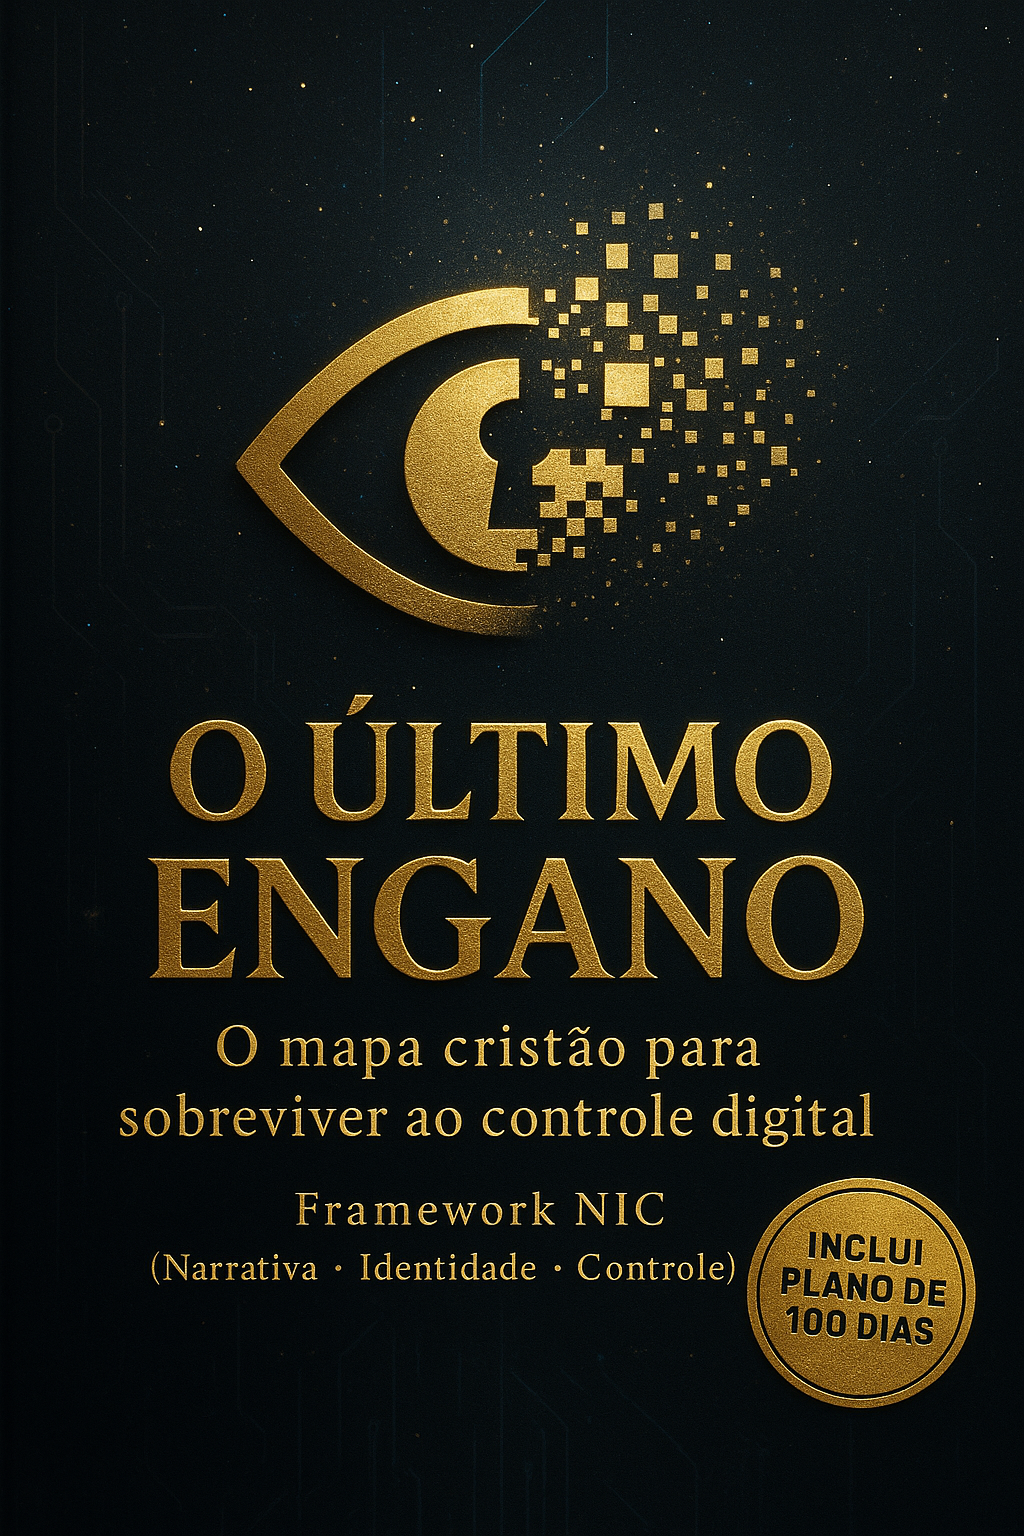
\includegraphics[width=\paperwidth,height=\paperheight]{img/capa.png}
\restoregeometry
\endgroup
\clearpage

\maketitle
\clearpage
\thispagestyle{empty}
\vspace*{0.6\textheight}
{\centering \sffamily\Large O Último Engano\par}
\clearpage

\clearpage
\thispagestyle{empty}
\vspace*{0.55\textheight}
\noindent\footnotesize © \the\year\ Andrey Alencar Quadros. Todos os direitos reservados.\\
Proibida a reprodução total ou parcial sem autorização do autor.\\
ISBN: \_\_\_\_\_\_\_\_ \hfill Primeira edição.\\[1ex]
Projeto editorial: \textit{Apocalipse Tecnológico}. Composto em EB Garamond e Source Sans Pro.
\clearpage

\chapter*{Dedicatória}
Para [nome], que me ensinou a esperar o Cordeiro.

\chapter*{Epígrafe}
\begin{flushright}
``E conhecerão a verdade, e a verdade os libertará.''\\
\textit{João 8:32}
\end{flushright}

\chapter*{Agradecimentos}
A Deus, à minha família e à igreja que caminha comigo. Aos leitores que desejam discernir os tempos sem perder a esperança.

% \chapter*{Prefácio}
% (Opcional — por convidado)
 % opcional

\chapter*{Introdução}
\markboth{Introdução}{Introdução}

Este livro nasceu de uma convicção simples: \textbf{Jesus reina}, e portanto é possível viver com \textbf{prudência, esperança e fidelidade} em meio a sistemas cada vez mais digitais, centralizados e persuasivos. 
O que chamamos aqui de \textit{apocalipse tecnológico} não é um ``novo evangelho'', mas a \textbf{convergência} entre velhos padrões bíblicos de idolatria e \textbf{ferramentas} modernas que amplificam \emph{narrativas}, \emph{identidades} e \emph{controles}.

\section*{A grande ideia: NIC}
A espinha dorsal deste livro é o \textbf{framework NIC} --- \textit{Narrativa, Identidade e Controle}. 
Ele aparece em boxes, exercícios e checklists ao longo dos capítulos:
\begin{nicbox}
\begin{itemize}[leftmargin=*,noitemsep]
  \item \textbf{Narrativa} (\emph{o que é verdade?}) --- quem conta a história e como ela é legitimada.
  \item \textbf{Identidade} (\emph{quem eu sou?}) --- selos, marcas, nomes, pertencimento.
  \item \textbf{Controle} (\emph{o que posso fazer?}) --- portas de compra e venda, permissões, coerções.
\end{itemize}
\end{nicbox}
Quando o leitor aprender a enxergar NIC nos textos bíblicos \emph{e} nos sistemas digitais, ganhará uma bússola simples para tempos confusos.

\section*{Para quem escrevo}
Para cristãos comuns, líderes e profissionais de tecnologia que desejam discernir os sinais do nosso tempo sem pânico nem ingenuidade. \textbf{Não} peço que você concorde com todas as minhas leituras, apenas que verifique \textit{com a Bíblia aberta} e aplique com amor à sua família e igreja.

\section*{Como usar este livro}
Cada capítulo segue uma arquitetura constante: \textit{vinheta de abertura} (história curta), \textit{mapa bíblico enxuto}, \textit{NIC aplicado}, \textit{ferramenta/checklist} e \textit{perguntas para grupo}. Feche cada capítulo com uma \textbf{pequena prática} na semana: são passos modestos que, somados, formam um Plano de 100 Dias (reunido no apêndice).

\section*{Sobre apócrifos e debates escatológicos}
Cito eventualmente literatura judaica do período intertestamentário (p.\,ex., 1~Enoque) como \textit{contexto histórico}, não como autoridade canônica. Quanto às posições escatológicas (premilenismo, amilenismo, pós-milenismo), priorizo o que é \textbf{essencial} e apologio por caridade no que é \textbf{secundário}. O leitor encontrará um mapa honesto no final do livro.

\section*{Convites}
\begin{checklist}[title={Antes de começar}]
\begin{itemize}[leftmargin=*,noitemsep]
  \item Separe uma Bíblia de papel e um caderno. Desligue notificações durante a leitura.
  \item Comprometa-se com \textbf{30 minutos semanais} para ler Daniel 7, Mateus 24, 2~Tessalonicenses~2 e Apocalipse 1.
  \item Crie no caderno três abas: \textbf{N} (Narrativa), \textbf{I} (Identidade), \textbf{C} (Controle).
  \item Combine com alguém de sua igreja de lerem juntos um capítulo por semana.
\end{itemize}
\end{checklist}

Seja bem-vindo. O objetivo não é “vencer discussões na internet”, mas \textbf{cuidar de gente} sob o senhorio de Cristo. Quando a cidade apagar, que sua casa brilhe.


\tableofcontents

% ---------------------------------- TEXTUAIS ----------------------------------
\mainmatter

% Prólogo (não numerado na TOC com addcontentsline)
\chapter*{Prólogo — 48 horas de blackout}
\addcontentsline{toc}{chapter}{Prólogo — 48 horas de blackout}

A cidade apagou às 18h42 de uma terça-feira quente. Primeiro veio o silêncio estranho dos aparelhos desligando ao mesmo tempo. Depois, um coro de apitos dos nobreaks. A luz piscou, morreu. A tela do celular continuou brilhando por alguns minutos, mas o 4G sumiu em seguida. As mensagens pararam de ser entregues. O aplicativo do banco travou; o \textit{Pix} não ia, o cartão não passava. A portaria do prédio comunicou pelo interfone que os elevadores foram travados por segurança.

Às 19h15, você foi à janela. Uma rua inteira de janelas escuras e lanternas vacilantes. O mercado da esquina levantou meia porta para ventilar. Algumas pessoas corriam com sacolas para dentro de casa. Outras discutiam com o caixa, que não sabia como registrar as compras sem o sistema. Um vizinho tentou usar dinheiro vivo. O caixa não tinha troco.

No primeiro dia, a maior dificuldade foi \textbf{Narrativa}. Ninguém sabia ao certo o que estava acontecendo. O boato mais compartilhado no prédio: “\textit{É ataque cibernético}”. Outro: “\textit{É racionamento de energia}”. Um terceiro: “\textit{É o fim do mundo}”. Sem internet, o condomínio improvisou um quadro de avisos no hall com recados escritos à mão. As pessoas queriam \textit{uma} história que explicasse o caos.

Na manhã seguinte, faltou água no 10º andar: as bombas do prédio dependem de energia. A geladeira começou a descongelar. O segundo golpe foi de \textbf{Identidade}. Sem internet, logins não funcionavam; sem login, muitos serviços não reconheciam você. Um vizinho preso do lado de fora do trabalho não conseguiu passar pela catraca porque o acesso é biométrico na nuvem. Outro não conseguiu “abrir um chamado” para a empresa de luz: o app exigia autenticação de dois fatores\footnote{Dois fatores são ótimos---quando existem os dois fatores.}.

À noite, a tensão subiu. Para vários comércios, o problema se tornou \textbf{Controle}. Sem pagamentos digitais, sem sistema de estoque, sem segurança privada (as câmeras também caíram), alguns fecharam as portas. Outros venderam apenas por anotações em cadernos “para acertar depois”. A padaria limitou a compra de pães por família. Alguém sugeriu um “rateio” de água para o prédio. Um grupo marcou oração no térreo: sem som, sem telão, sem QR Code; só vozes.

\begin{nicbox}
\textbf{Três perguntas NIC para um blackout:}\\[-1ex]
\begin{enumerate}[leftmargin=*,nosep]
  \item \textbf{Narrativa} --- Quem define a história quando os algoritmos emudecem? Como discernir boato de verdade?
  \item \textbf{Identidade} --- Quem somos sem nossos logins, QR Codes e senhas? O que nos confirma quando o sistema não confirma?
  \item \textbf{Controle} --- O que fazemos quando as portas de compra e venda fecham? Como praticar justiça e generosidade quando a escassez bate?
\end{enumerate}
\end{nicbox}

No final das primeiras 24 horas, as famílias que estavam mais tranquilas tinham três traços simples: um plano de comunicação offline, alguma reserva básica (água, gás, dinheiro trocado) e uma comunidade próxima (parentes, vizinhos, igreja). Nada heroico; só \textit{prudência}.

\begin{checklist}[title={Primeiras 24 horas: ações simples}]
\begin{itemize}[leftmargin=*,noitemsep]
  \item Combine \textit{pontos de encontro} e \textit{horários} de checagem presencial com a família.
  \item Desligue tomadas críticas para proteger equipamentos quando a energia voltar.
  \item Separe água potável e identifique recipientes de uso sanitário.
  \item Organize alimentos que não exigem refrigeração; priorize o que pode estragar.
  \item Faça um \textit{mapa de vizinhança}: quem tem necessidades especiais? Quem pode ajudar?
  \item Anote no papel contatos essenciais (família, líderes, serviços).
  \item Defina um \textit{horário fixo} de oração e leitura breve da Palavra.
\end{itemize}
\end{checklist}

No final das 48 horas, a luz voltou em ondas, bairro a bairro. As redes sociais retornaram como uma torrente. As narrativas competiam outra vez, mas agora com gráficos e especialistas. Você respirou aliviado, mas percebeu que algo tinha mudado: o \emph{mundo}---não apenas os aparelhos---ficara frágil.

Este livro começa aqui. Não para alimentar pânico, mas para formar \textbf{prudência, esperança e fidelidade}. Ao longo das próximas páginas, vamos mapear como tecnologia e Apocalipse se cruzam nas \textbf{três frentes NIC}:
\begin{enumerate}[leftmargin=*,nosep]
  \item \textbf{Narrativa} (\textit{verdade}) --- quando a “imagem que fala” cria mundos plausíveis;
  \item \textbf{Identidade} (\textit{quem sou}) --- quando somos reduzidos a perfis e credenciais;
  \item \textbf{Controle} (\textit{o que posso fazer}) --- quando portas de compra e venda são programáveis.
\end{enumerate}

E faremos isso de modo bíblico e prático: com critérios de leitura, cenários realistas, checklists e disciplinas espirituais. Porque, quando a cidade apaga, \textit{a igreja acende}. E quando a nuvem falha, o Cordeiro permanece.

\bigskip
\noindent\textit{Próximo capítulo: Como ler Apocalipse sem delirar.}


\part{Fundamentos que não quebram}
\chapter{Como ler Apocalipse sem delirar}
Apocalipse é \textbf{revelação de Jesus Cristo} (\emph{apokálypsis Iēsou Christou}, Ap 1:1), não um código secreto para iniciados. Antes de falar sobre “marca”, “besta” ou “imagem que fala”, precisamos alinhar \textit{como} ler o livro sem cair em extremos de ingenuidade ou paranoia.

\section{O centro que não muda}
A chave de leitura é a pessoa e a obra de Cristo: “o testemunho de Jesus é o espírito da profecia” (Ap 19:10). Tudo aponta para o Cordeiro que venceu (Ap 5). Se um esquema “escatológico” move você para longe de Cristo, está torto.

\section{Gênero e símbolos: o que é o que?}
Apocalipse combina carta, profecia e literatura apocalíptica. Isso explica a \textbf{densidade simbólica}: dragões, estrelas, taças, chifres. Símbolos não são \emph{menos} reais; apontam para realidades \emph{maiores}. A regra é deixar a própria Escritura interpretar seus sinais:
\begin{itemize}[leftmargin=*,noitemsep]
  \item Olhe \textbf{para trás} (\textit{intertexto}): Daniel (2, 7, 9), Ezequiel, Zacarias.
  \item Olhe \textbf{para dentro}: quando Apocalipse explica o símbolo (p.\,ex., “as sete lâmpadas são os sete espíritos de Deus”). 
  \item Olhe \textbf{para frente} com sobriedade: aplique, mas não force a tecnologia a “caber” no texto.
\end{itemize}

\section{Quatro escolas de leitura (e uma via integradora)}
Há leituras \textit{preterista} (muito já se cumpriu no séc. I), \textit{historicista} (cumprimentos ao longo da história), \textit{futurista} (ênfase no fim literal) e \textit{idealista} (princípios atemporais). Em vez de brigar, vamos \textbf{integrar o melhor de cada}:
\begin{itemize}[leftmargin=*,noitemsep]
  \item Do \textbf{preterismo}: contexto real das igrejas da Ásia e do Império.
  \item Do \textbf{historicismo}: consciência de ciclos e padrões.
  \item Do \textbf{futurismo}: esperança concreta na volta de Cristo.
  \item Do \textbf{idealismo}: aplicação para \textit{todas} as gerações.
\end{itemize}

\begin{nicbox}
\textbf{Regra das Três Janelas}\\
\textit{Texto original} (o que significou) \ $\rightarrow$ \ \textit{Cristo} (quem Ele é) \ $\rightarrow$ \ \textit{Igreja hoje} (como obedecer).
\end{nicbox}

\section{Erros comuns e antídotos práticos}
\begin{checklist}
\begin{itemize}[leftmargin=*,noitemsep]
  \item \textbf{Datismo}: marcar datas. \emph{Antídoto}: vigiar e trabalhar (Mt 24).
  \item \textbf{Jornalismo-escatológico}: forçar toda manchete no texto. \emph{Antídoto}: voltar ao contexto bíblico.
  \item \textbf{Tecnofobia ou tecnoeuforia}: demonizar ou idolatrar tecnologia. \emph{Antídoto}: tecnologia como ferramenta sob o senhorio de Cristo.
  \item \textbf{Desligamento pastoral}: especular sem cuidar de gente. \emph{Antídoto}: edificar a igreja local primeiro.
\end{itemize}
\end{checklist}

\section{Mini-exegese: a ``imagem da besta'' e a ``marca''}
Ap 13 descreve uma \textbf{imagem que recebe fôlego e fala} e um \textbf{sinal} sem o qual ninguém pode comprar ou vender. O texto aponta para \textit{adoração} e \textit{lealdade} (culto), antes de qualquer tecnologia específica. As tecnologias atuais (IA generativa, biometria, moedas programáveis) \textit{podem} servir como meios para coerção, mas o centro permanece espiritual: \emph{quem adoramos}.

\section{Aplicando o framework NIC à leitura bíblica}
Pergunte em cada texto:
\begin{itemize}[leftmargin=*,noitemsep]
  \item \textbf{Narrativa} --- Que história sobre o mundo está sendo contada? Quem a legitima?
  \item \textbf{Identidade} --- Quem recebe um nome, um selo, um livro onde o nome é escrito?
  \item \textbf{Controle} --- Quais portas se abrem ou fecham? Quem define quem participa da vida econômica?
\end{itemize}

\begin{nicbox}
\textbf{Exercício rápido}\\
Leia Ap 2--3 (cartas às igrejas) e marque com canetas de três cores: falas sobre \textbf{verdade} (N), \textbf{pertencimento} (I) e \textbf{perseverança/autoridade} (C). Discuta o que cada igreja precisava ouvir.
\end{nicbox}

\section{Perguntas para grupos pequenos}
\begin{itemize}[leftmargin=*,noitemsep]
  \item Que \textit{narrativas} rivais disputam seu coração hoje? Como testá-las biblicamente?
  \item Em que momentos sua \textit{identidade} foi reduzida a performance ou perfil?
  \item Que práticas sua família/igreja pode adotar quando o \textit{controle} digital falhar?
\end{itemize}

\section{Checklist do capítulo}
\begin{checklist}
\begin{itemize}[leftmargin=*,noitemsep]
  \item Reafirme: Jesus é o centro (Ap 1; 5; 19:10).
  \item Decida uma \textbf{tradução bíblica} de referência e uma \textbf{Bíblia de estudo} confiável.
  \item Crie um caderno de notas com três abas: N (Narrativa), I (Identidade), C (Controle).
  \item Marque 30 minutos semanais para ler Daniel 7, Mateus 24, 2 Tessalonicenses 2 e Apocalipse 1.
\end{itemize}
\end{checklist}

\bigskip
\noindent\textit{Próximo capítulo: Graça, fé e perseverança --- o combustível da fidelidade no fim dos tempos.}

\chapter{Graça, fé e perseverança}
\label{cap:graca_fe}
\noindent\textit{Vinheta.} Um jovem recém-batizado decide “limpar o feed” e reduzir o tempo de tela. Na primeira semana, vai bem. Na segunda, desliza. Sente culpa, então tenta “compensar” com regras rígidas e promessas que não cumpre. Ao final do mês, conclui: “\textit{Eu não dou conta}”. 
O problema não é a \emph{falta de ferramenta}, é a \textbf{fonte} de onde ele opera. O evangelho oferece essa fonte: \textbf{graça} que recebemos pela \textbf{fé}, gerando \textbf{perseverança}.

\section{O motor da fidelidade}
O Novo Testamento é claro: “\emph{Pela graça sois salvos, mediante a fé; e isto não vem de vós, é dom de Deus}” (Ef~2:8--9). A vida cristã \textit{começa} e \textit{continua} assim: graça recebida, fé que confia, amor que trabalha (Gl~5:6). Em tempos de pressão tecnológica (vigilância, persuasão, coerção), quem persevera não é o “mais disciplinado”, mas quem \textbf{permanece em Cristo} (Jo~15).

\section{Graça que educa, não que desculpa}
Graça não é tolerância ao pecado; é o poder de Deus que nos \textbf{educa} (Tt~2:11--12). Ela nos treina a renunciar “impiedade e paixões mundanas” e a viver “sensata, justa e piedosamente” \textit{neste século}. Isso inclui nosso trato com telas, algoritmos e conveniências.

\section{Fé que confia em meio ao ruído}
Fé bíblica não é pensamento positivo, é \textbf{confiança relacional} em Deus revelado em Cristo. Em um ambiente onde muitas “verdades” disputam sua atenção, a fé pratica duas posturas: \textit{ouvir} (Palavra) e \textit{obedecer} (passos concretos). A Palavra ancora a narrativa; a obediência realinha a identidade.

\section{Perseverança: a arte de continuar}
Perseverança é permanecer sob o peso (\emph{hypomonē}). Não é teimosia cega; é \textbf{esperança aplicada} (Rm~5:3--5; Tg~1:2--4). Em termos práticos, a perseverança cristã se sustenta em três meios de graça ordinários: \textit{Palavra, oração e comunhão}. Tecnologia pode ajudar (lembretes, leituras, calendário), mas não substitui \textbf{pessoas} e \textbf{liturgias} simples.

\section{NIC aplicado: por que graça, fé e perseverança importam no digital}
\begin{nicbox}
\textbf{Narrativa} --- A graça reescreve a história: não somos \emph{o que entregamos}, somos \emph{os que recebemos}.\\
\textbf{Identidade} --- A fé nos ancora em Cristo: não somos perfis; somos filhos adotivos.\\
\textbf{Controle} --- A perseverança responde à coerção: quando portas fecham, respondemos com fidelidade criativa.
\end{nicbox}

\section{Práticas que funcionam em 15 minutos por dia}
\begin{checklist}
\begin{itemize}[leftmargin=*,noitemsep]
  \item \textbf{Lectio breve} (5 min): leia um salmo em voz alta; sublinhe um verbo de Deus.
  \item \textbf{Oração dirigida} (5 min): agradeça por 3 graças recebidas no dia; peça 1 ajuda concreta.
  \item \textbf{Passo pequeno} (5 min): um ato de obediência mensurável (ligar para alguém, pedir perdão, agendar encontro).
\end{itemize}
\end{checklist}

\section{Higiene de telas que nasce da graça}
Não começamos pelo “não pode”; começamos pelo “\textit{a quem pertencemos}”. A partir disso, implementamos limites \emph{simples}:
\begin{checklist}[title={Regra de bolso (7 dias)}]
\begin{itemize}[leftmargin=*,noitemsep]
  \item Um \textbf{primeiro olhar} do dia para a Palavra, não para o celular.
  \item Uma \textbf{janela de tela} definida (p.\,ex., 8h–21h) e o celular dorme fora do quarto.
  \item Uma \textbf{refeição sem tela} por dia com conversa e oração curta.
  \item Um \textbf{dia de sabá digital} (6h sem redes sociais).
\end{itemize}
\end{checklist}

\section{Perguntas para grupos pequenos}
\begin{itemize}[leftmargin=*,noitemsep]
  \item Onde você tem tentado “vencer” no braço aquilo que só a graça pode operar?
  \item Que prática de 15 minutos por dia você pode iniciar esta semana?
  \item Como sua igreja pode facilitar perseverança (pequenos grupos, leitura comunitária, mentorias)?
\end{itemize}

\bigskip
\noindent\textit{Próximo capítulo: Verdade em tempos de deepfake --- discernindo narrativas e testando espíritos.}

\chapter{Verdade em tempos de \textit{deepfake}}
\noindent\textit{Vinheta.} Um vídeo explode nos grupos da igreja: o pastor ``confessa'' ter abandonado a fé. A voz, a entonação, tudo parece dele. Em minutos, membros chocados começam a sair dos ministérios. Só no fim do dia alguém descobre: era um \textit{deepfake}. O dano, porém, já aconteceu.

\section{Mapa bíblico (curto e claro)}
\begin{itemize}[leftmargin=*,noitemsep]
  \item \textbf{Discernir espíritos} (1~Jo~4:1): ``\textit{provai os espíritos}'' --- existe verdade e mentira \emph{espiritual}.
  \item \textbf{Sinais enganadores} (Mt~24:24; 2~Ts~2:9--12): “\textit{grandes sinais e prodígios}” e “\textit{mentiras}” que parecem plausíveis.
  \item \textbf{Prudência na fala} (Pv~18:17; Tg~1:19): a primeira versão da história costuma parecer certa \emph{até} ser examinada.
  \item \textbf{Estabilidade em Cristo} (Ef~4:14): não ser “\textit{levado por todo vento de doutrina}”.
\end{itemize}

\section{Como a mentira digital opera (4 mecanismos simples)}
\begin{itemize}[leftmargin=*,noitemsep]
  \item \textbf{Velocidade}: a mentira chega antes; a correção vem tarde.
  \item \textbf{Verossimilhança}: \textit{deepfake}/IA emprestam aparência de realidade.
  \item \textbf{Vínculo}: quando toca emoções/identidade, fixamos a narrativa.
  \item \textbf{Vantagem}: algoritmos amplificam o que retém atenção (nem sempre o que é verdade).
\end{itemize}

\begin{nicbox}
\textbf{NIC aplicado}\\
\textbf{Narrativa}: quem conta a história e que evidências apresenta?\\
\textbf{Identidade}: por que isso me atinge (tribo, medo, indignação)?\\
\textbf{Controle}: que ação imediata essa peça tenta provocar em mim (compartilhar, comprar, pressionar, agredir)?
\end{nicbox}

\section{Ferramenta 1 — Teste ``4P'' da verdade prática}
Use antes de reagir ou compartilhar:
\begin{checklist}[title={4P: Provedor, Prova, Palavra, Propósito}]
\begin{itemize}[leftmargin=*,noitemsep]
  \item \textbf{Provedor}: quem publicou primeiro? é rastreável? tem histórico?
  \item \textbf{Prova}: há \emph{fonte primária} (documento, áudio/vídeo original, data/autor)? há \emph{corroboração} independente?
  \item \textbf{Palavra}: o conteúdo afronta princípios claros da Escritura (calúnia, maledicência, incitação)?
  \item \textbf{Propósito}: qual a ação desejada (compartilhar no impulso, doar, votar, humilhar)? a pressa é o sinal de alerta.
\end{itemize}
\end{checklist}

\section{Ferramenta 2 — Checklist de 60 segundos (para leigos ocupados)}
\begin{checklist}
\begin{itemize}[leftmargin=*,noitemsep]
  \item \textbf{Pausa 10s}: respire. Emoção alta = julgamento baixo.
  \item \textbf{Olho no autor}: perfil novo, sem histórico, ou com nome parecido com oficial?
  \item \textbf{Data/hora}: conteúdo antigo reempacotado?
  \item \textbf{Foto/vídeo}: parece IA? sombras/olhos/dentes não naturais, piscadas estranhas, legendas desalinhadas.
  \item \textbf{Procure 2 confirmações}: busque o mesmo fato em fontes diferentes.
  \item \textbf{Não compartilhe no escuro}: se você não checaria pessoalmente no púlpito, não poste no grupo da igreja.
\end{itemize}
\end{checklist}

\section{Ferramenta 3 — Protocolo para líderes (quando o alvo é a sua igreja)}
\begin{checklist}[title={Resposta em 3 passos},breakable]
\begin{itemize}[leftmargin=*,noitemsep]
  \item \textbf{Reconheça rápido}: ``Vimos o conteúdo X. Estamos verificando. Não compartilhem.''
  \item \textbf{Verifique técnico e pastoral}: equipe de mídia checa autenticidade; equipe pastoral cuida das pessoas atingidas.
  \item \textbf{Responda com luz}: publique \emph{fatos} e \emph{caminhos de cuidado} (horários de reunião, aconselhamento, Q\&A).
\end{itemize}
\end{checklist}

\section{Mini-exegese: ``testar os espíritos'' no século XXI}
1~Jo~4:1 não ficou obsoleto porque temos cadeias de blocos e marcas d'água. O teste inclui \emph{doutrina} (Cristo encarnado), \emph{ética} (fruto do Espírito) e \emph{comunhão} (o ensino que permanece com a igreja). Ferramentas digitais ajudam, mas não substituem testemunho e caráter. O mal moderno continua sendo o velho mal: mentira contra a verdade de Cristo.

\section{Práticas semanais que criam anticorpos}
\begin{checklist}
\begin{itemize}[leftmargin=*,noitemsep]
  \item \textbf{Liturgia da verdade} (10 min): ler em voz alta Jo~8:31--32; orar pedindo amor à verdade mais que à razão.
  \item \textbf{Ritual de checagem} (1 noite/semana): escolher uma notícia viral e aplicar o 4P em família ou pequeno grupo.
  \item \textbf{Jejum de encaminhar} (7 dias): zero \emph{forward} sem checagem dupla.
\end{itemize}
\end{checklist}

\section{Perguntas para grupos pequenos}
\begin{itemize}[leftmargin=*,noitemsep]
  \item Que narrativa recente você compartilhou e depois precisou corrigir? O que te apressou?
  \item Em que tipo de conteúdo você percebe maior vulnerabilidade (medo, política, fofoca religiosa)?
  \item Como aplicar o protocolo de líderes à realidade da sua igreja?
\end{itemize}

\bigskip
\noindent\textit{Próximo capítulo: Esperança que não pode ser hackeada --- por que a vitória do Cordeiro sustenta os nossos pés.}

\chapter{Esperança que não pode ser hackeada}
\noindent\textit{Vinheta.} Na terceira noite do blackout, sem Wi-Fi e sem luz, uma igreja pequena se reúne no pátio. Um violão, vozes cansadas, crianças correndo. Alguém lê Ap 21: ``\emph{Eis que faço novas todas as coisas}''. Não mudou a rede; mudou o povo. Eles voltam para casa mais leves.

\section{Mapa bíblico (o eixo da esperança)}
\begin{itemize}[leftmargin=*,noitemsep]
  \item \textbf{O Cordeiro venceu} (Ap~5): a história não está sem autor.
  \item \textbf{Juízos com propósito} (Ap~8--16): revelar, corrigir, salvar (Rm~2:4--5).
  \item \textbf{Queda da Babilônia} (Ap~18): ídolos caem; Cristo permanece.
  \item \textbf{Nova criação} (Ap~21--22): Deus com o seu povo; fim da lágrima e da morte.
\end{itemize}

\section{Esperança cristã \emph{vs.} otimismo tecnológico}
Esperança não é \textbf{otimismo}. Otimismo diz: ``vai dar certo porque a curva de inovação sobe''. Esperança diz: ``\textit{Cristo reina}, ainda que a curva desça''. O primeiro depende de \emph{tendências}; o segundo, de \emph{promessas}.

\section{Como a esperança opera na prática}
\begin{itemize}[leftmargin=*,noitemsep]
  \item \textbf{Afeto}: aprende a \emph{desejar} a cidade por vir (Hb~11:10).
  \item \textbf{Ação}: trabalha aqui e agora (Jr~29:7; 1~Co~15:58).
  \item \textbf{Âncora}: volta-se sempre ao Cordeiro (Heb~6:19; Ap~5).
\end{itemize}

\section{Mini-exegese: juízo não é pânico}
Os selos, trombetas e taças são dramáticos, mas não aleatórios. Eles desmascaram ídolos e chamam ao arrependimento. Ler Apocalipse com esperança significa \textbf{reconhecer a justiça de Deus} e \textbf{abraçar sua paciência} (2~Pe~3:9), sem cinismo nem desespero.

\begin{nicbox}
\textbf{NIC da esperança}\\
\textbf{Narrativa}: a história é do Cordeiro.\\
\textbf{Identidade}: somos selados (Ap~7) --- não perfis descartáveis.\\
\textbf{Controle}: mesmo quando portas se fecham, Cristo abre a porta da perseverança (Ap~3:8).
\end{nicbox}

\section{Práticas que alimentam esperança}
\begin{checklist}
\begin{itemize}[leftmargin=*,noitemsep]
  \item \textbf{Salmos na mesa} (5 min): ler um salmo por refeição principal em voz alta.
  \item \textbf{Boletim de gratidão} (1/semana): a família lista 3 sinais do cuidado de Deus.
  \item \textbf{Visita curta} (quinzenal): encorajar alguém aflito com Ap~21:1--5.
  \item \textbf{Ofertar tempo} (mensal): servir alguém sem reciprocidade possível.
\end{itemize}
\end{checklist}

\section{Perguntas para grupos pequenos}
\begin{itemize}[leftmargin=*,noitemsep]
  \item Que \textit{otimismo} você precisa confessar como \emph{idolatria} tecnológica?
  \item Em qual promessa bíblica você precisa se ancorar nesta estação?
  \item Como sua igreja pode encarnar Ap~21 em pequenos gestos na cidade?
\end{itemize}

\bigskip
\noindent\textit{Próximo capítulo: A imagem que fala --- IA, culto e a idolatria da conveniência.}


\part{A Máquina do Engano}
\chapter{A imagem que fala}
\noindent\textit{Vinheta.} Um culto on-line de alta produção passa a mostrar, em realidade aumentada, uma ``presença'' que responde orações em tempo real, com voz sintética e holograma. As pessoas choram, doam, compartilham. Mas aquilo não é Deus. É \textbf{engenharia de adoração}.

\section{Mapa bíblico}
\begin{itemize}[leftmargin=*,noitemsep]
  \item \textbf{A imagem que recebe fôlego e fala} (Ap~13:15): um artefato mediando culto e coerção.
  \item \textbf{Ídolos que têm boca e não falam} (Sl~115; Is~44): a ironia antiga reaparece com esteroides digitais.
  \item \textbf{Verdadeiro culto} (Jo~4:23--24; Rm~12:1): em espírito e em verdade; corpo como sacrifício vivo.
\end{itemize}

\section{IA generativa: por que é diferente desta vez}
\begin{itemize}[leftmargin=*,noitemsep]
  \item \textbf{Produção barata de plausibilidade}: texto, voz, imagem e vídeo sob demanda.
  \item \textbf{Personalização total}: cada fiel recebe uma ``liturgia'' sob medida.
  \item \textbf{Velocidade de milagre}: respostas instantâneas criam sensação de ``poder''.
  \item \textbf{Meio que vira mensagem}: a forma tecnológica molda a expectativa espiritual.
\end{itemize}

\section{O risco da \emph{idolatria da conveniência}}
Quando o culto vira produto e a presença de Deus é confundida com uma \textbf{experiência fluida}, a conveniência cobra \textbf{lealdade}. É mais fácil obedecer à interface do que ao Senhor. \textbf{Lei 1 do Engano Digital}: \emph{conveniência sempre cobra lealdade}.

\begin{nicbox}
\textbf{NIC aplicado}\\
\textbf{Narrativa}: ``Deus quer que você se sinta sempre bem'' \emph{vs.} ``Deus quer torná-lo santo''.\\
\textbf{Identidade}: consumidor de conteúdos religiosos \emph{vs.} adorador que se oferece a Deus.\\
\textbf{Controle}: plataformas como novos ``átrios'' que abrem e fecham portas de visibilidade e monetização.
\end{nicbox}

\section{Mini-exegese: o que \emph{não} forçar no texto}
Ap~13 não exige um \emph{modelo tecnológico} específico. Exige discernir \textbf{adoração + coerção}. IA, hologramas e realidades mistas podem ser \emph{meios} de idolatria, mas a raiz é sempre a \textbf{lealdade do coração}. 

\section{Ferramenta — Auditoria de culto (30 minutos para líderes)}
\begin{checklist}[title={Perguntas para o conselho/produção}]
\begin{itemize}[leftmargin=*,noitemsep]
  \item Nosso culto facilita \textbf{participação} ou apenas \textbf{consumo}? 
  \item Usamos tecnologia para \textbf{clareza e serviço} ou para \textbf{deslumbrar e prender}? 
  \item Nossa liturgia forma \textbf{adoradores} (Jo~4) ou \textbf{clientes}?
  \item O que permanece se perdermos \textbf{luzes, telas e automação} por 30 dias?
\end{itemize}
\end{checklist}

\section{Práticas para a igreja local}
\begin{checklist}
\begin{itemize}[leftmargin=*,noitemsep]
  \item \textbf{Elementos irredutíveis}: leitura pública da Palavra, oração congregacional, ceia/batismo, cânticos bíblicos, generosidade.
  \item \textbf{Tecnologia serva}: projetor e som para \emph{clareza}; sem pirotecnia vazia.
  \item \textbf{Liturgias caseiras}: culto doméstico semanal sem tela (Salmo, breve Palavra, oração).
  \item \textbf{Transparência}: publique orçamento e critérios de produção; corte o que não serve à edificação.
\end{itemize}
\end{checklist}

\section{Perguntas para grupos pequenos}
\begin{itemize}[leftmargin=*,noitemsep]
  \item Em que momentos você confunde \textit{experiência} com \textit{presença de Deus}?
  \item Que tecnologia precisa ser recolocada no seu culto como \textbf{serva}, não como \textbf{senhora}?
  \item O que sua igreja manteria se perdesse a infraestrutura por um mês?
\end{itemize}

\bigskip
\noindent\textit{Próximo capítulo: Profetas do algoritmo --- recomendação, bolhas e fabricação de consenso.}

\chapter{Profetas do algoritmo}
\noindent\textit{Vinheta.} Você abre o celular ``só por cinco minutos''. Uma sequência perfeita de vídeos curtos prende seu olhar. Quando percebe, perdeu quarenta. Não foi acaso. Foi \textbf{curadoria algorítmica}: um profeta moderno que anuncia, dia e noite, o que você ``precisa'' ver.

\section{Mapa bíblico}
\begin{itemize}[leftmargin=*,noitemsep]
  \item \textbf{Falsos profetas e sinais} (Mt~24:11,24): falas sedutoras que desviam o coração.
  \item \textbf{Coceira nos ouvidos} (2~Tm~4:3--4): preferir narrativas que confortam desejos.
  \item \textbf{Cativo a Cristo, não à tela} (2~Co~10:5): levar todo pensamento cativo à obediência de Cristo.
  \item \textbf{Atenção como mordomia} (Ef~5:15--16): remir o tempo, porque os dias são maus.
\end{itemize}

\section{Como funciona a recomendação (sem jargão)}
Algoritmos aprendem com seus \textit{sinais de engajamento}: tempo de tela, curtidas, comentários, pausas, replays. Eles combinam dados seus com dados de milhões para prever o que mais prolonga sua permanência. \textbf{Objetivo}: maximizar atenção. \textbf{Efeito colateral}: reforço de vieses e \textbf{bolhas} que parecem profecias personalizadas.

\section{Quatro dinâmicas do ``profeta'' algorítmico}
\begin{itemize}[leftmargin=*,noitemsep]
  \item \textbf{Atração}: entrega conteúdos emocionalmente carregados (\emph{medo}, \emph{ira}, \emph{vaidade}).
  \item \textbf{Aderência}: recompensa você por voltar; cria \emph{rituais} de checagem.
  \item \textbf{Aderência tribal}: conecta você a grupos com linguagem interna (``nós vs. eles'').
  \item \textbf{Autoridade emergente}: o \emph{feed} vira referência: ``se está em alta, deve ser verdade''.
\end{itemize}

\begin{nicbox}
\textbf{NIC aplicado}\\
\textbf{Narrativa}: a plataforma narra o mundo a partir do seu engajamento, não da realidade.\\
\textbf{Identidade}: você é reduzido a um \emph{perfil preditivo}.\\
\textbf{Controle}: seu comportamento é \emph{nudgeado} (empurrado) em microdecisões diárias.
\end{nicbox}

\section{Mini-exegese: o poder da \textit{coceira} (2~Tm~4:3)}
Paulo descreve uma \textbf{demanda por narrativas} que se ajustem a desejos. Os ``profetas do algoritmo'' entregam precisamente isso: uma liturgia de confirmação. O antídoto continua sendo o mesmo: \textbf{Palavra saudável}, \textbf{sã doutrina}, \textbf{vida comunitária} e \textbf{sobriedade}.

\section{Ferramenta --- Higiene informacional em 7 passos}
\begin{checklist}
\begin{itemize}[leftmargin=*,noitemsep]
  \item \textbf{Limpeza de fonte}: siga menos, siga melhor. Desative notificações push não essenciais.
  \item \textbf{Janelas de consumo}: horários fixos (p.\,ex., 12h30 e 19h) --- fora disso, o app fica \emph{off}.
  \item \textbf{Tempo de tela}: limite por app (p.\,ex., 20--30 min/dia); senha administrada por alguém de confiança.
  \item \textbf{Variedade intencional}: insira fontes que discordam de você (2:1 entre concordância e dissonância).
  \item \textbf{Ritual 4P} (cap.~3): Provedor, Prova, Palavra, Propósito antes de compartilhar.
  \item \textbf{Desintoxicação semanal}: 12 horas sem \emph{feed}; use tempo para conversas e leitura bíblica.
  \item \textbf{Comunhão} acima de consumo: substitua 1 hora de rolagem por 1 encontro real.
\end{itemize}
\end{checklist}

\section{Ferramenta --- Plano 3 camadas (pessoa, família, igreja)}
\begin{checklist}[title={Protocolos práticos},breakable]
\begin{itemize}[leftmargin=*,noitemsep]
  \item \textbf{Pessoal}: escolha 2 horários fixos de ver redes; \emph{mute} palavras-gatilho; desinstale um app por 30 dias.
  \item \textbf{Família}: aparelho carregando fora do quarto; 1 refeição/dia sem tela; noite de checagem 4P (quinzenal).
  \item \textbf{Igreja}: encoraje \emph{estudos de caso} mensais (uma fake viral dissecada); política de comunicação clara para crises.
\end{itemize}
\end{checklist}

\section{Evite dois extremos}
\begin{itemize}[leftmargin=*,noitemsep]
  \item \textbf{Tecnofobia}: demonizar toda plataforma --- perde-se o campo missionário.
  \item \textbf{Tecnoeuforia}: abraçar toda novidade --- vira-se refém do \emph{hype}.
\end{itemize}
Empurre a tecnologia para o seu lugar: \textbf{serva}. Coloque Cristo no Dele: \textbf{Senhor}.

\section{Perguntas para grupos pequenos}
\begin{itemize}[leftmargin=*,noitemsep]
  \item Quais conteúdos mais sequestram sua atenção (medo, escândalo, vaidade)? Por quê?
  \item O que você \textit{pode} remover esta semana (notificação, app, horário gatilho)?
  \item Que política de crise sua igreja precisa escrever antes da próxima tempestade de boatos?
\end{itemize}

\bigskip
\noindent\textit{Próximo capítulo: Identidade programável --- IDs digitais, biometria e reputação.}

\chapter{Identidade programável}
\noindent\textit{Vinheta.} No balcão da farmácia, a atendente aponta para um tablet: ``\emph{Olhe para a câmera, por favor.}'' Reconhecimento facial para liberar o desconto do convênio. Mais tarde, ao tentar acessar um serviço público, o aplicativo pede uma prova de vida por selfie. À noite, o banco envia um aviso: ``\emph{Por segurança, seu limite foi reduzido até nova verificação.}'' Em um só dia, sua \textbf{identidade} virou uma sequência de \emph{checks} --- e qualquer falha virou \textbf{bloqueio}.

\section{Mapa bíblico}
\begin{itemize}[leftmargin=*,noitemsep]
  \item \textbf{Selo e pertencimento} (Ef~1:13; Ap~7:2--3): Deus \emph{sela} seu povo --- identidade recebida, não negociada.
  \item \textbf{Nome e lealdade} (Ap~13:16--17; 14:1): \emph{marcas} que distinguem quem adoramos.
  \item \textbf{Justiça com o frágil} (Is~1:17; Tg~1:27): proteger vulneráveis de exclusão e injustiça sistêmica.
\end{itemize}

\section{O que é identidade programável}
Chamamos de \textbf{identidade programável} o conjunto de \emph{credenciais digitais} (CPF/IDs, senhas, biometria, \emph{tokens}, reputações) que podem ser verificadas por máquinas e conectadas a \emph{permissões} (entrar, comprar, votar, viajar) e \emph{restrições} (limites, bloqueios). É útil, mas cria \textbf{dependências} e \textbf{portas} que alguém controla.

\section{Exemplos práticos (Brasil)}
\begin{itemize}[leftmargin=*,noitemsep]
  \item \textbf{Conta gov.br}: acesso unificado a serviços públicos, com níveis de verificação que podem incluir \emph{selfie} e validações biométricas.
  \item \textbf{Documentos digitais}: CNH/CRLV digitais e outras carteiras em aplicativos oficiais; sincronização com bases do Estado.
  \item \textbf{Biometria em serviços privados}: bancos, telecom e saúde usando selfie/voz/face para liberar operações e descontos.
  \item \textbf{Pagamentos rápidos + KYC}: transferências instantâneas combinadas a cadastros \emph{conheça seu cliente} --- identidade e transação se aproximam.
\end{itemize}

\section{Exemplos práticos (internacional)}
\begin{itemize}[leftmargin=*,noitemsep]
  \item \textbf{Carteiras de identidade digitais na Europa}: iniciativas públicas para credenciais verificáveis entre países e setores.
  \item \textbf{Índia (Aadhaar)}: número de identidade com biometria, usado para benefícios e autenticações amplas.
  \item \textbf{Sistemas de reputação e pontuação}: modelos \emph{públicos e privados} que atrelam comportamento/risco a acesso a serviços.
  \item \textbf{Autenticação passkey/biométrica}: grandes plataformas movendo logins para chaves criptográficas e biometria de dispositivo.
\end{itemize}

\section{Dinâmicas de risco (o que costuma dar problema)}
\begin{itemize}[leftmargin=*,noitemsep]
  \item \textbf{Falsos negativos}: \emph{você} não passa na validação (voz rouca, luz ruim, câmera ruim) e perde acesso.
  \item \textbf{Vazamentos e correlação}: bases de dados diferentes conectadas criando perfis extensos sem seu controle.
  \item \textbf{Bloqueios automáticos}: regras antifraude que punem inocentes (conta congelada, compra negada, cadastro travado).
  \item \textbf{Exclusão silenciosa}: idosos, pessoas com deficiência, áreas sem conectividade --- quem não entra no fluxo digital fica à margem.
\end{itemize}

\begin{nicbox}
\textbf{NIC aplicado}\\
\textbf{Narrativa}: ``segurança total'' justifica coleta e verificação contínuas.\\
\textbf{Identidade}: reduzida a \emph{fatores de autenticação} (algo que você tem/é/sabe).\\
\textbf{Controle}: portas de acesso podem ser abertas/fechadas por políticas e algoritmos --- às vezes sem interlocutor humano.
\end{nicbox}

\section{Mini-exegese: o selo que liberta (Ef 1:13 vs. marcas que escravizam)}
O \textbf{selo do Espírito} é dom que \emph{confirma} nossa filiação e liberdade em Cristo. Já a \textbf{marca coercitiva} de Ap~13 liga \emph{adoração} a \emph{controle econômico}. A tecnologia pode \emph{instrumentalizar} esse controle, mas o eixo é sempre \textbf{lealdade do coração}. Por isso, formamos pessoas cuja identidade não depende do ``login'' do mundo.

\section{Ferramenta --- Protocolo pessoal de identidade (15 minutos)}
\begin{checklist}
\begin{itemize}[leftmargin=*,noitemsep]
  \item \textbf{Mapa de contas}: liste serviços críticos (banco, e-mail, nuvem, gov., saúde) e quem tem acesso de recuperação.
  \item \textbf{Autenticação com sabedoria}: use autenticação de dois fatores com app físico/OTP; evite SMS como único método.
  \item \textbf{Plano B offline}: guarde \emph{backup} de códigos de recuperação em local físico seguro; anote contatos essenciais no papel.
  \item \textbf{Higiene de dados}: revise permissões de aplicativos (câmera, microfone, localização); revogue o que não usa.
  \item \textbf{Sinais de alerta}: se pedir \emph{selfie} toda hora, questione; se negar sem recurso, documente e escale.
\end{itemize}
\end{checklist}

\section{Ferramenta --- Quando a validação falha (passo a passo)}
\begin{checklist}[title={Recuperação de acesso},breakable]
\begin{itemize}[leftmargin=*,noitemsep]
  \item \textbf{Evidência}: registre tela e horário do erro; anote protocolos.
  \item \textbf{Redundância}: tente \emph{canal alternativo} (agência física, telefone verificado, e-mail secundário).
  \item \textbf{Interlocutor humano}: peça atendimento que \emph{não dependa} da mesma biometria que falhou.
  \item \textbf{Proteção financeira}: se banco, solicite carta de \emph{não reconhecimento} e congele transações suspeitas.
  \item \textbf{Comunidade}: avise família/igreja para suporte prático (pagamentos, deslocamento, documentos).
\end{itemize}
\end{checklist}

\section{Ferramenta --- Igreja e organizações (política de identidade justa)}
\begin{checklist}[title={Princípios para líderes}]
\begin{itemize}[leftmargin=*,noitemsep]
  \item \textbf{Mínimo necessário}: colete o mínimo de dados para servir; evite armazenar documentos sensíveis.
  6
  \item \textbf{Alternativa analógica}: ofereça caminho sem smartphone/biometria para membros idosos ou vulneráveis.
  \item \textbf{Transparência}: explique por que coleta, por quanto tempo, e quem tem acesso.
  \item \textbf{Resposta a incidentes}: procedimento claro para vazamentos e perdas de acesso dos membros.
\end{itemize}
\end{checklist}

\section{Perguntas para grupos pequenos}
\begin{itemize}[leftmargin=*,noitemsep]
  \item Já ficou ``travado'' por causa de uma validação que falhou? Como resolveu?
  \item Que dados você pode \textbf{minimizar} hoje (revogar, excluir, desinstalar)?
  \item Como sua igreja pode acolher quem não consegue ``passar na máquina''?
\end{itemize}

\bigskip
\noindent\textit{Próximo capítulo: Marca, moedas e portas de compra e venda --- quando conveniência vira coerção.}

\chapter{Marca, moedas e portas de compra e venda}
\noindent\textit{Vinheta.} Um pequeno comércio do bairro passa a aceitar apenas pagamentos digitais por ``segurança''. Na semana seguinte, o banco atualiza os termos: ``\emph{Para sua proteção, certas categorias terão limites automáticos}''. Um mês depois, uma política pública oferece \emph{descontos programáveis} para quem compra em parceiros credenciados. Conveniência? Sim. Mas uma pergunta NIC acende: \textbf{quem controla a porta}?

\section{Mapa bíblico}
\begin{itemize}[leftmargin=*,noitemsep]
  \item \textbf{Portas econômicas} (Ap~13:16--17): sem o sinal, ``ninguém compre ou venda'' --- \emph{culto} e \emph{coerção} se tocam.
  \item \textbf{Justiça e pesos honestos} (Pv~11:1; Mq~6:11): Deus se importa com as \emph{regras do mercado}.
  \item \textbf{Generosidade na escassez} (At~11:27--30; 2~Co~8): a igreja responde ao controle com \emph{partilha e fidelidade}.
\end{itemize}

\section{CBDCs e dinheiro programável (em linguagem simples)}
\textbf{CBDC} é moeda digital emitida pelo \emph{banco central}. Pode ser \textbf{de atacado} (entre bancos) ou \textbf{de varejo} (para o público). ``Programável'' significa que \emph{regras de uso} podem ser embutidas no pagamento (p.\,ex., validade, destinos permitidos, descontos condicionais). Benefícios prometidos: eficiência, inclusão, combate a fraude. Riscos: \textbf{portas} de compra e venda \emph{centralmente} controláveis, com erros e abusos possíveis.

\section{Panorama 2025 (resumo, sem alarmismo)}
\begin{itemize}[leftmargin=*,noitemsep]
  \item \textbf{Lançados} (uso doméstico em curso): Bahamas (Sand Dollar), Jamaica (Jam-Dex), Nigéria (eNaira).
  \item \textbf{Pilotos relevantes}: China (e-CNY, maior piloto), Índia (e-rupee, varejo em piloto), Hong Kong (e-HKD, piloto em fases), projetos de atacado para \emph{pagamentos transfronteiriços} (ex.: mBridge). 
  \item \textbf{Europa}: debate legislativo sobre \emph{euro digital}; Suécia concluiu pilotos técnicos do \emph{e-krona} e segue avaliando.
  \item \textbf{Brasil}: \textbf{Drex} --- arquitetura com \emph{camada de atacado} (liquidação em dinheiro do BC) e \emph{depósitos tokenizados} para o varejo (não é ``carteira do BC'' para o público). Foco: tokenização, eficiência e contratos inteligentes.
\end{itemize}

\begin{nicbox}
\textbf{NIC aplicado}\\
\textbf{Narrativa}: ``mais segurança e inclusão'' --- verdadeiro em partes, mas incompleto se omitir riscos de governança.\\
\textbf{Identidade}: carteira \emph{KYC} e reputações podem redefinir quem ``pode'' transacionar.\\
\textbf{Controle}: portas de compra/venda podem ser abertas/fechadas por políticas, algoritmos e \emph{parceiros} de plataforma.
\end{nicbox}

\section{Lei 2 do Engano Digital}
\textbf{Quem controla a porta, controla o culto}. Quando acesso econômico depende de \emph{conformidade comportamental}, a “porta” vira \textbf{altar}. O perigo não é a \emph{tecnologia} em si, mas a \textbf{lealdade} que ela exige para funcionar.

\section{Cenários práticos (o bom, o difícil e o perigoso)}
\begin{itemize}[leftmargin=*,noitemsep]
  \item \textbf{O bom}: benefícios pagos instantaneamente a quem mais precisa; \emph{cashback} para merenda escolar; taxas menores para microcomércios.
  \item \textbf{O difícil}: \emph{falsos negativos} e bloqueios automáticos deixam inocentes sem acesso por dias.
  \item \textbf{O perigoso}: \emph{restrições geográficas} e \emph{categorias proibidas} (ou “desincentivadas”) definidas de modo opaco; exclusão silenciosa de dissidentes ou vulneráveis.
\end{itemize}

\section{Brasil em foco (Drex, Pix e tokenização)}
\begin{itemize}[leftmargin=*,noitemsep]
  \item \textbf{Pix} segue como infraestrutura-chave para pagamentos instantâneos; tende a integrar-se com arranjos mais complexos (ex.: liquidação de ativos tokenizados).
  \item \textbf{Drex} propõe uma \emph{camada de atacado} com dinheiro do BC para liquidação e uma \emph{camada de varejo} por depósitos tokenizados via bancos --- com \textbf{contratos inteligentes} para programar regras \emph{no ativo}, não \emph{no cidadão}.
  \item \textbf{Implicação pastoral}: excelente para baratear \emph{boas} regras (fraude, conciliação); risco se “regras de vida” forem embutidas no dinheiro (uso, destino, prazo).
\end{itemize}

\section{Exemplos internacionais (instantâneo 2025)}
\begin{itemize}[leftmargin=*,noitemsep]
  \item \textbf{China (e-CNY)}: piloto em grande escala, incluindo transporte, varejo e eventos; discussão sobre uso transfronteiriço.
  \item \textbf{Índia (e-rupee)}: piloto de varejo com expansão para bancos e \emph{fintechs}; planos de explorar casos transfronteiriços.
  \item \textbf{Hong Kong (e-HKD)}: piloto por fases (\emph{e-HKD+}) com testes de atacado e varejo integrados.
  \item \textbf{mBridge (transfronteiriço)}: plataforma multi-BCs (China, Hong Kong, Tailândia, EAU; adesões adicionais) em estágio de produto mínimo viável para pagamentos internacionais.
  \item \textbf{Europa}: \emph{euro digital} em discussão política e desenho técnico; foco em privacidade e limites de saldo.
\end{itemize}

\section{Ferramenta --- ``Portas'' do seu orçamento (auditoria de 30 minutos)}
\begin{checklist}
\begin{itemize}[leftmargin=*,noitemsep]
  \item \textbf{Multi-rails}: tenha ao menos \emph{3 vias} de pagamento (Pix/cartão/dinheiro). Dinheiro vivo para emergências.
  \item \textbf{Reserva de liquidez}: 2--4 semanas de despesas essenciais em formas \emph{acessíveis offline}.
  \item \textbf{Documentos e prova de vida}: guarde alternativas \emph{não biométricas} para validações (cartório, senhas de recuperação).
  \item \textbf{Comércio local}: incentive negócios do bairro a manter ao menos um meio de pagamento \emph{fora de nuvem}.
  \item \textbf{Caridade organizada}: fundo da igreja para socorrer bloqueios temporários (alimentos, remédios, transporte).
\end{itemize}
\end{checklist}

\section{Ferramenta --- Política de generosidade e objeção de consciência (igreja e famílias)}
\begin{checklist}[title={Princípios práticos}]
\begin{itemize}[leftmargin=*,noitemsep]
  \item \textbf{Transparência}: explique por que usam certos meios de pagamento e quais dados são coletados.
  \item \textbf{Alternativa digna}: sempre ofereça \emph{um caminho} sem app ou biometria.
  \item \textbf{Limites}: recuse \emph{condições morais} embutidas no dinheiro; priorize \emph{servir pessoas} acima de metas algorítmicas.
  \item \textbf{Resiliência comunitária}: crie uma rede de apoio para membros que sofrerem \emph{bloqueios} inesperados.
\end{itemize}
\end{checklist}

\section{Perguntas para grupos pequenos}
\begin{itemize}[leftmargin=*,noitemsep]
  \item Onde sua família está \textbf{superdependente} de uma única ``porta'' de pagamento?
  \item Que \textbf{política de alternativa analógica} sua igreja precisa escrever esta semana?
  \item Em que ponto \emph{conveniência} começou a exigir \emph{lealdade} no seu coração?
\end{itemize}

\bigskip
\noindent\textit{Próximo capítulo: Transumanismo --- ``sereis como Deus?'' bio/neurotecnologia e limites éticos.}

\chapter{Transumanismo: ``sereis como Deus?'' (o que já é real e comprovado)}
\noindent\textit{Vinheta.} Uma mulher com doença hematológica grave recebe uma única infusão de células reprogramadas fora do corpo e, meses depois, não volta mais ao hospital. Um idoso com Parkinson volta a caminhar com eletrodos implantados. Uma criança nasce ouvindo graças a um implante coclear. Não são promessas de ficção científica. São \textbf{intervenções reais}, com \textbf{evidência robusta}.

\section{Mapa bíblico}
\begin{itemize}[leftmargin=*,noitemsep]
  \item \textbf{Criação e limites} (Gn~1--2): dignidade do corpo e mandato cultural (cuidar, desenvolver, ordenar).
  \item \textbf{Queda e hybris} (Gn~3; 11): a tentação de ``\emph{sereis como Deus}'' e a torre (Babel) como símbolo de autonomia arrogante.
  \item \textbf{Cura e compaixão} (Mt~9:35; Lc~10:25--37): a medicina como expressão de amor ao próximo.
  \item \textbf{Sabedoria e prudência} (Pv~1:7; Tg~1:5): discernimento para abraçar o bem e recusar o mal.
\end{itemize}

\section{O que já tem \emph{provas} sólidas}
\subsection*{1) Edição/terapia genética \& celular (doença, não ``superpoder'')}
\begin{itemize}[leftmargin=*,noitemsep]
  \item \textbf{CRISPR e afins}: terapias aprovadas para doenças hematológicas específicas; outros alvos em fases avançadas. Foco: \emph{correção ou compensação} de mutações, não ``melhoramento'' de pessoas saudáveis.
  \item \textbf{Terapias gênicas não editoras}: vetores virais para repor genes (ex.: distúrbios hereditários da visão, musculares e metabólicos) com estudos clínicos publicados.
  \item \textbf{Terapias celulares}: CAR-T (reprogramação de linfócitos) para certos cânceres hematológicos, com remissões duradouras em subgrupos.
\end{itemize}

\subsection*{2) Neurotecnologia \& interfaces cérebro-dispositivo}
\begin{itemize}[leftmargin=*,noitemsep]
  \item \textbf{Estimulação cerebral profunda (DBS)}: padrão estabelecido para Parkinson e distonia (\emph{evidence-based}, décadas de acompanhamento).
  \item \textbf{Implantes auditivos} (coclear) e \textbf{retinais} (casos selecionados): restauração parcial de função sensorial.
  \item \textbf{Interfaces neurais para comunicação/movimento}: dispositivos invasivos e minimamente invasivos permitindo \emph{cursor/teclado} e controle de próteses em pacientes com paralisia, com publicações revisadas por pares.
  \item \textbf{Neuroestimulação periférica/medular}: alívio de dor crônica e \emph{reaprendizado motor} em lesões específicas.
\end{itemize}

\subsection*{3) Próteses, exoesqueletos \& biomateriais}
\begin{itemize}[leftmargin=*,noitemsep]
  \item \textbf{Próteses mioelétricas} com controle fino (sensores musculares/neurais) e \textbf{feedback háptico} em pesquisa aplicada.
  \item \textbf{Exoesqueletos} assistivos para marcha e reabilitação.
  \item \textbf{Biomateriais} e impressões 3D para órteses e peças ósseas personalizadas.
\end{itemize}

\subsection*{4) Medicina da longevidade (o que tem base vs. hype)}
\begin{itemize}[leftmargin=*,noitemsep]
  \item \textbf{O que tem base}: controle de fatores de risco, sono, exercício resistido, dieta adequada, vacinas, rastreios; terapias para doenças específicas.
  \item \textbf{O que está em estudo}: senolíticos, reprogramação parcial, marcadores epigenéticos --- promissor, mas ainda sem consenso clínico para uso amplo.
  \item \textbf{O que é hype}: “pílulas universais de longevidade”, \emph{upload} de mente, promessas sem ensaios robustos.
\end{itemize}

\section{O que \emph{não} tem boa prova (por enquanto)}
\begin{itemize}[leftmargin=*,noitemsep]
  \item \textbf{Melhoramento humano} generalizado (força, memória, QI) por edição genética em \emph{germes} (germline) --- forte rejeição ética e ausência de segurança/eficácia.
  \item \textbf{Imortalidade digital} (\emph{mind uploading}) --- especulação filosófica/tecnológica sem validação científica.
  \item \textbf{Reversão ampla do envelhecimento} em humanos --- resultados \emph{pré-clínicos} não equivalem a benefício clínico comprovado.
\end{itemize}

\section{NIC aplicado ao transumanismo}
\begin{nicbox}
\textbf{Narrativa} --- de ``cura e cuidado'' para ``otimização e poder''. Pergunte: qual história está guiando a decisão?\\
\textbf{Identidade} --- do ``corpo recebido'' para o ``projeto editável''. Quem eu sou se posso mudar tudo?\\
\textbf{Controle} --- quem decide \emph{quem} recebe o quê, \emph{quando} e \emph{segundo que} critérios?
\end{nicbox}

\section{Mini-exegese: ``sereis como Deus'' (Gn 3) e os ``dias de Noé'' (Gn 6)}
A tentação não é a \emph{ferramenta}, é o \textbf{tronodeus} do coração: autonomia sem adoração, poder sem serviço. ``Dias de Noé'' evocam \textbf{corrupção generalizada} e \textbf{violência}, mais do que um mecanismo biotecnológico específico. Nossa leitura cristã celebra a medicina que \textbf{serve} o próximo e recusa a tecnologia que \textbf{substitui} Deus.

\section{Princípios éticos claros (para profissionais e pacientes)}
\begin{checklist}[title={Linhas de orientação},breakable]
\begin{itemize}[leftmargin=*,noitemsep]
  \item \textbf{Finalidade}: priorizar \emph{cura/cuidado} sobre \emph{melhoramento competitivo}.
  \item \textbf{Consentimento e verdade}: riscos reais, benefícios realistas; sem promessas mágicas.
  \item \textbf{Justiça}: evitar que tecnologias salvadoras virem \emph{privilégios de poucos}.
  \item \textbf{Limites} (\emph{germline}, quimeras, manipulações identitárias): \textbf{não} cruzar fronteiras sem consenso científico, ético e legal sólido.
  \item \textbf{Objeção de consciência}: direito de dizer ``não'' a procedimentos que violem convicções informadas.
\end{itemize}
\end{checklist}

\section{Ferramenta --- Decisão clínica informada (famílias e igrejas)}
\begin{checklist}
\begin{itemize}[leftmargin=*,noitemsep]
  \item Traga um \textbf{médico de confiança} para traduzir o jargão (peça \emph{ensaios clínicos} e \emph{nível de evidência}).
  \item Pergunte: o objetivo é \textbf{tratar} ou \textbf{otimizar}? Qual o \textbf{benefício absoluto} e os \textbf{efeitos colaterais}?
  \item Avalie \textbf{custo e acesso}: existe cobertura? há alternativa padrão de cuidado?
  \item Considere \textbf{valores e propósito}: esta decisão me torna \emph{mais fiel} e \emph{mais útil} ao próximo?
  \item Ore com sua comunidade e \textbf{documente} a decisão para evitar pressão/culpa futura.
\end{itemize}
\end{checklist}

\section{Perguntas para grupos pequenos}
\begin{itemize}[leftmargin=*,noitemsep]
  \item Onde você percebe \textbf{hype} substituindo \textbf{prudência} nas conversas sobre tecnologia e saúde?
  \item Que \textbf{história} está moldando sua visão: cura que serve, ou poder que exibe?
  \item Como sua igreja pode apoiar membros em decisões médicas complexas sem julgamento e sem ingenuidade?
\end{itemize}

\bigskip
\noindent\textit{Próximo capítulo: Arquitetura da Babilônia 2.0 --- cidades inteligentes, IoT e vigilância ubíqua.}


\part{Guerra silenciosa por Narrativa, Identidade e Controle}
\chapter{Arquitetura da Babilônia 2.0}
\noindent\textit{Vinheta.} Uma tempestade derruba torres de transmissão e fecha o principal acesso rodoviário à capital por 48 horas. O porto reduz operação. As operadoras racionam sinal. Supermercados lotam; \textit{Pix} oscila, cartões recusam. A padaria anuncia: ``\emph{Hoje só dinheiro e quantidade limitada.}'' O problema \emph{não} é maldade de pessoas. É \textbf{dependência de infraestrutura} --- elétrica, logística, telecom, pagamentos --- \emph{em cascata}.

\section{Mapa bíblico}
\begin{itemize}[leftmargin=*,noitemsep]
  \item \textbf{Cidade e poder} (Gn 11): Babel como símbolo de concentração sem Deus.
  \item \textbf{Comércio e queda} (Ap 18): quando a economia vira ídolo, ``\emph{em uma hora chegou a tua ruína}''.
  \item \textbf{Prudência comunitária} (Gn 41): José prepara a cidade para escassez com \textbf{planejamento}.
  \item \textbf{Mordomia e cuidado} (Pv 6:6--8; 1~Tm 5:8): prover para os seus, com diligência.
  \item \textbf{Paz da cidade} (Jr 29:7): trabalhar pelo bem comum, mesmo no exílio.
\end{itemize}

\section{Segurança pública \emph{vs.} privacidade (resumo honesto)}
Cidades ``inteligentes'' usam sensores, câmeras, análise de dados e automação. Benefícios: \textbf{resposta rápida} a emergências, trânsito mais fluido, melhor uso de recursos. Riscos: \textbf{vigilância massiva}, \textbf{perfilização} e \textbf{abuso de dados}. Como cristãos, buscamos \textbf{ordem justa} sem render a liberdade do próximo a uma \emph{onisciência simulada}.

\begin{nicbox}
\textbf{NIC aplicado (segurança x privacidade)}\\
\textbf{Narrativa}: ``segurança absoluta'' costuma pedir \emph{silêncio} sobre trade-offs.\\
\textbf{Identidade}: moradores viram \emph{perfis de risco}.\\
\textbf{Controle}: regras automatizadas definem quem entra, circula e compra.
\end{nicbox}

\section{Dependência de infraestrutura (o foco deste capítulo)}
Pense a cidade como \textbf{cinco redes interdependentes}:
\begin{enumerate}[leftmargin=*,nosep]
  \item \textbf{Energia elétrica} (geração, transmissão, distribuição);
  \item \textbf{Telecomunicações} (móvel, fibra, data centers, cloud);
  \item \textbf{Água e saneamento} (captação, tratamento, bombeamento);
  \item \textbf{Logística e combustíveis} (portos, rodovias, armazéns, postos);
  \item \textbf{Pagamentos e comércio} (\emph{Pix}, cartões, TEF, ERPs, bancos).
\end{enumerate}
Quando \emph{uma} falha, costuma \textbf{puxar} as outras: sem energia, caem antenas e bombas; sem telecom, caem pagamentos; sem combustível, a logística trava; sem logística, o mercado esvazia.

\section{Cadeia alimentar urbana (do campo ao prato)}
\begin{itemize}[leftmargin=*,noitemsep]
  \item \textbf{Produção} $\rightarrow$ \textbf{atacadistas/centrais} $\rightarrow$ \textbf{transporte} $\rightarrow$ \textbf{varejo} $\rightarrow$ \textbf{consumidor}.
  \item Alimentos frescos têm \textbf{giro rápido} e \textbf{cadeia fria} (refrigeração) sensível a falhas.
  \item \textbf{Pagamentos e estoque} dependem de sistemas (ERPs, TEF, nuvem). Sem eles, muitos comércios ficam \emph{legal e tecnicamente} impedidos de operar.
\end{itemize}

\section{Cenários de falha (gatilhos e respostas)}
\subsection*{1) Queda prolongada de energia}
\begin{itemize}[leftmargin=*,noitemsep]
  \item \textbf{Gatilhos}: interrupções em vários bairros; retorno intermitente; comunicados de racionamento.
  \item \textbf{Resposta}: proteger equipamentos, priorizar alimentos perecíveis, usar gelo térmico/caixas, \textbf{evitar} geradores em ambientes fechados.
\end{itemize}

\subsection*{2) Falha de telecom/pagamentos}
\begin{itemize}[leftmargin=*,noitemsep]
  \item \textbf{Gatilhos}: \emph{Pix}/cartões instáveis; bancos e operadoras fora do ar; ERPs lentos/offline.
  \item \textbf{Resposta}: \textbf{dinheiro trocado}, recibos manuais, combinar comércios que vendem ``\emph{anotar para acertar}''; priorizar compras essenciais.
\end{itemize}

\subsection*{3) Logística e combustíveis}
\begin{itemize}[leftmargin=*,noitemsep]
  \item \textbf{Gatilhos}: bloqueios, greves, deslizamentos, portos/rodovias fechados; filas em postos.
  \item \textbf{Resposta}: reduzir deslocamentos, \textbf{carona solidária}, planejamento de consultas/viagens, uso racional de estoque doméstico.
\end{itemize}

\subsection*{4) Sistemas de comércio (software/ERP) indisponíveis}
\begin{itemize}[leftmargin=*,noitemsep]
  \item \textbf{Gatilhos}: quedas amplas de serviços em nuvem; varejo só em dinheiro; nota fiscal indisponível.
  \item \textbf{Resposta}: comprar em mercadinhos/bancas que operam manualmente; \textbf{evitar} grandes volumes e estocagem egoísta.
\end{itemize}

\subsection*{5) Evento climático extremo}
\begin{itemize}[leftmargin=*,noitemsep]
  \item \textbf{Gatilhos}: alertas meteorológicos, enchentes, geadas, ondas de calor.
  \item \textbf{Resposta}: água potável priorizada; abrigos e rotas seguras; medicamentos e documentos à mão.
\end{itemize}

\section{Ferramenta --- Auditoria de abastecimento do seu bairro (90 minutos)}
\begin{checklist}
\begin{itemize}[leftmargin=*,noitemsep]
  \item Liste \textbf{3 mercados}, \textbf{2 farmácias}, \textbf{1 padaria} e \textbf{1 açougue} acessíveis a pé.
  \item Verifique \textbf{formas de pagamento} aceitas e se operam \emph{manualmente} sem sistema.
  \item Identifique \textbf{feiras livres} e \textbf{cestas locais} (produtores da região).
  \item Conversem com gerentes: ``\emph{Se cair pagamento/energia, como vocês fazem?}''
  \item Mapeie \textbf{postos} e \textbf{oficinas} confiáveis no entorno.
\end{itemize}
\end{checklist}

\section{Ferramenta --- Plano doméstico 7/30 dias (essenciais reais)}
\begin{checklist}[title={Itens e hábitos},breakable]
\begin{itemize}[leftmargin=*,noitemsep]
  \item \textbf{Água}: reserve para 7 dias (regra prática: 3--4\,L por pessoa/dia para beber e preparo). Reponha e rode o estoque.
  \item \textbf{Alimentos}: básicos de \textbf{pronto preparo} (grãos, enlatados, frutas secas, aveia, leite em pó), abridor manual, gás/álcool/lenha seguros.
  \item \textbf{Saúde}: remédios contínuos + kit simples (analgésico, curativos), receitas impressas; itens infantis/idosos.
  \item \textbf{Energia e luz}: lanternas, pilhas, \emph{power banks} carregados, tomadas filtradas; se possuir gerador, uso \textbf{exclusivamente ventilado}.
  \item \textbf{Comunicação}: pontos de encontro, números \textbf{no papel}, rádio simples se possível.
  \item \textbf{Financeiro}: \textbf{dinheiro trocado}; registro manual de despesas; priorização de contas essenciais.
  \item \textbf{Documentos}: cópias físicas protegidas e digitais \emph{criptografadas}.
\end{itemize}
\end{checklist}

\section{Ferramenta --- Igreja/comunidade: mutualidade e mercado justo}
\begin{checklist}
\begin{itemize}[leftmargin=*,noitemsep]
  \item \textbf{Mapa de vizinhança}: quem é vulnerável? quem tem habilidades (mecânico, enfermeira, motorista)?
  \item \textbf{Rede de produtores}: conexão com agricultores/atacadistas para \emph{compra coletiva} quando o varejo fraquejar.
  \item \textbf{Cozinha solidária}: preparar refeições em escala quando faltar gás/energia na vizinhança (rodízio de casas).
  \item \textbf{Fundo de emergência}: ajuda rápida (alimentos, remédios, transporte) sem burocracia.
  \item \textbf{Comunicação impressa}: boletins com horários, orientações, endereços úteis.
\end{itemize}
\end{checklist}

\section{NIC aplicado (infraestrutura)}
\begin{nicbox}
\textbf{Narrativa}: “\emph{Sempre vai funcionar}” é crença, não garantia.\\
\textbf{Identidade}: somos mais que \emph{consumidores conectados}; somos \emph{corpo} que se cuida.\\
\textbf{Controle}: portas tecnológicas podem falhar ou fechar; a igreja abre portas de \textbf{generosidade}.
\end{nicbox}

\section{Perguntas para grupos pequenos}
\begin{itemize}[leftmargin=*,noitemsep]
  \item Quais as \textbf{duas dependências} críticas da sua casa hoje? Como reduzir?
  \item Qual o \textbf{plano de pagamento} da sua família quando \emph{Pix}/cartões falharem?
  \item Quem na sua rua precisa de ajuda imediata em um apagão? Quem pode ajudar?
\end{itemize}

\bigskip
\noindent\textit{Próximo capítulo: Crise, colapso e poder --- ciberataques, cadeias de suprimento e lei marcial informacional.}

\chapter{Crise, colapso e poder}
\noindent\textit{Vinheta.} Numa terça-feira comum, um ataque de \emph{ransomware} paralisa uma operadora de logística que atende supermercados, farmácias e postos. Caminhões param, sistemas de estoque caem, prazos explodem. Em poucas horas, não é ``uma empresa com problema'': é a cidade que fica mais \textbf{frágil}. A narrativa oficial pede calma; nos bastidores, decisões emergenciais definem quem recebe primeiro. \textbf{Poder} flui para quem controla as chaves.

\section{Mapa bíblico}
\begin{itemize}[leftmargin=*,noitemsep]
  \item \textbf{Poder e serviço} (Mc~10:42--45): governar como quem serve, não dominar.
  \item \textbf{Cidades que caem} (Ap~18): cadeias econômicas desmoronam ``\emph{numa hora}''.
  \item \textbf{Vigilância e sobriedade} (1~Pe~5:8; Mt~24): atenção e perseverança, sem pânico.
  \item \textbf{Justiça e verdade} (Pv~21:3; Ef~4:25): transparência e retidão em tempos de confusão.
\end{itemize}

\section{Três motores de crise}
\begin{itemize}[leftmargin=*,noitemsep]
  \item \textbf{Ciberataques}: \emph{ransomware}, DDoS, comprometimento de cadeia de suprimentos de software.
  \item \textbf{Choques físicos/logísticos}: clima extremo, greves, bloqueios, acidentes em portos/rodovias.
  \item \textbf{Crises de confiança/narrativa}: boatos, \emph{deepfakes}, decisões opacas que geram corrida a mercados/bancos.
\end{itemize}

\section{Lei marcial informacional (o que é e como lidar)}
Chamamos de \textbf{lei marcial informacional} o conjunto de \emph{restrições emergenciais} sobre comunicação e acesso a plataformas durante crises (para conter pânico, golpes ou desordem). Pode incluir limitação de \emph{upload}, derrubada de conteúdos, prioridade a canais oficiais e suspensão temporária de certos recursos.
\begin{itemize}[leftmargin=*,noitemsep]
  \item \textbf{Risco}: decisões opacas, abuso de poder, silenciamento de alertas legítimos.
  \item \textbf{Resposta cristã}: buscar o bem comum sem idolatrar a ordem; falar verdade com prudência; garantir \emph{canais alternativos} para cuidado.
\end{itemize}

\begin{nicbox}
\textbf{NIC aplicado}\\
\textbf{Narrativa}: quem define o que é ``oficial''? há prestação de contas?\\
\textbf{Identidade}: quem ganha o rótulo de ``confiável'' ou ``problemático''?\\
\textbf{Controle}: quem recebe \emph{prioridade} de recursos (combustível, tráfego, reposição)? por quais critérios?
\end{nicbox}

\section{Quadro de sinais precoces (o que acompanhar \emph{antes} de faltar no mercado)}
\begin{checklist}[title={Indicadores práticos para leigos}]
\begin{itemize}[leftmargin=*,noitemsep]
  \item \textbf{Energia}: comunicados de racionamento, avisos de manutenção extensa, quedas em múltiplos bairros.
  \item \textbf{Telecom}: falhas simultâneas de mais de uma operadora; latência anormal; apps bancários instáveis.
  \item \textbf{Logística}: notícias de porto/rodovia fechados; filas em postos; relatos de falta de insumos (gás, diesel).
  \item \textbf{Comércio}: limite de compras por item; “apenas dinheiro”; prateleiras recorrentes vazias no \emph{básico} (arroz, leite, ovos).
  \item \textbf{Saúde}: aumento de espera em UPA/UBS; falta de medicamentos comuns; suspensão de exames eletivos.
  \item \textbf{Narrativa}: mudança de tom oficial para ``\emph{pequenas restrições temporárias}'' sem prazo claro.
\end{itemize}
\end{checklist}

\section{Cenários críticos e contramedidas}
\subsection*{1) Ciberataque a pagamentos/ERP}
\begin{itemize}[leftmargin=*,noitemsep]
  \item \textbf{Efeitos}: cartão/TEF fora; notas fiscais indisponíveis; conciliação quebrada.
  \item \textbf{Contramedidas}: dinheiro trocado; recibo manual; compras pequenas; priorize comércios que operam sem sistema.
\end{itemize}

\subsection*{2) Paralisação logística (portos/rodovias)}
\begin{itemize}[leftmargin=*,noitemsep]
  \item \textbf{Efeitos}: desabastecimento pontual (combustível, hortifrúti); alta de preços.
  \item \textbf{Contramedidas}: reduzir deslocamentos; compras fracionadas; feiras locais; cozinhas compartilhadas.
\end{itemize}

\subsection*{3) Corte de energia em larga escala}
\begin{itemize}[leftmargin=*,noitemsep]
  \item \textbf{Efeitos}: cadeia fria comprometida; bombas d'água paradas; telecom instável.
  \item \textbf{Contramedidas}: priorize perecíveis; água estocada; \emph{power banks}; vizinhança solidária.
\end{itemize}

\subsection*{4) Lei marcial informacional (restrição de canais)}
\begin{itemize}[leftmargin=*,noitemsep]
  \item \textbf{Efeitos}: difícil verificar boatos; canais oficiais saturados; confusão.
  \item \textbf{Contramedidas}: pontos de encontro; líderes de quarteirão; boletins impressos; rádio/comunicação simples.
\end{itemize}

\section{Protocolo 48--72 horas (família e igreja)}
\begin{checklist}[title={Passo a passo objetivo},breakable]
\begin{itemize}[leftmargin=*,noitemsep]
  \item \textbf{Hora 0--6}: confirmar segurança de todos; desligar equipamentos sensíveis; definir ponto de encontro e horário de checagem.
  \item \textbf{Hora 6--12}: água e alimentos essenciais; contactar vizinhos vulneráveis; separar dinheiro trocado; organizar medicações.
  \item \textbf{Hora 12--24}: racionar uso de bateria; cozinhar perecíveis; registrar ocorrências (fotos, anotações) e \textbf{não} espalhar boatos.
  \item \textbf{Hora 24--48}: reavaliar estoque; planejar revezamento de tarefas (cozinhar, buscar água, vigiar); boletim simples para o grupo/igreja.
  \item \textbf{Hora 48--72}: se persistir, ativar redes de apoio (compra coletiva de alimentos, acolhimento de famílias); culto doméstico/comunitário de encorajamento.
\end{itemize}
\end{checklist}

\section{Ferramenta --- Política de crise da igreja (uma página)}
\begin{checklist}
\begin{itemize}[leftmargin=*,noitemsep]
  \item \textbf{Cadastre líderes de quarteirão}: 1 contato por rua/condomínio.
  \item \textbf{Defina ponto físico de referência}: templo ou casa estratégica.
  \item \textbf{Escreva mensagens-tipo}: ``Reconhecemos X; estamos fazendo Y; pedimos Z; horário do próximo boletim.''
  \item \textbf{Critérios de auxílio}: prioridades para idosos, crianças, doentes e trabalhadores essenciais.
  \item \textbf{Transparência}: prestação de contas pública de doações e gastos.
\end{itemize}
\end{checklist}

\section{Postura do discípulo em tempos de colapso}
\begin{itemize}[leftmargin=*,noitemsep]
  \item \textbf{Coração}: esperança firme (cap.~4), sem cinismo.
  \item \textbf{Cabeça}: informação verificada (cap.~3 e 6), sem credulidade.
  \item \textbf{Mãos}: serviço prático (cap.~10), sem egoísmo.
\end{itemize}

\section{Perguntas para grupos pequenos}
\begin{itemize}[leftmargin=*,noitemsep]
  \item Quais \textbf{sinais precoces} você já percebeu na sua cidade nos últimos meses?
  \item Sua família consegue cumprir este \textbf{protocolo 48--72h} hoje? O que falta?
  \item Como sua igreja pode decidir \textbf{critérios de auxílio} justos antes da próxima crise?
\end{itemize}

\bigskip
\noindent\textit{Próximo capítulo: O Anticristo --- paródia da Trindade e o mínimo que todo cristão precisa saber.}

\chapter{O Anticristo: paródia da Trindade (o mínimo que todo cristão precisa saber)}
\noindent\textit{Vinheta.} Uma coalizão improvável de poder político, propaganda e milagre digital dá voz a uma liderança mundial ``pacificadora''. O mundo aplaude; a igreja se divide. Alguns veem oportunidade; outros, perigo. Em meio ao ruído, a pergunta simples: \textbf{o que a Bíblia afirma com clareza} e o que é \textbf{especulação plausível}?

\section{Mapa bíblico (núcleo consensual)}
\begin{itemize}[leftmargin=*,noitemsep]
  \item \textbf{Daniel 7--8; 9; 11--12}: reinos sucessivos, um poder arrogante que exalta a si mesmo, persegue santos e profana o culto.
  \item \textbf{2 Tessalonicenses 2}: ``\emph{o homem da iniquidade}'' (ou ``sem lei'') exalta-se como Deus, com \emph{sinais de mentira}; há um \emph{restritor} e uma revelação final.
  \item \textbf{Apocalipse 13; 17; 19}: \textit{paródia da Trindade}: Dragão (paródia do Pai), Besta do Mar (paródia do Filho, poder político) e Falso Profeta/Besta da Terra (paródia do Espírito, propaganda/milagres) — levando à adoração e à \textbf{coerção econômica}.
\end{itemize}

\section{Quatro não negociáveis (linha de base)}
\begin{checklist}
\begin{itemize}[leftmargin=*,noitemsep]
  \item \textbf{Pessoalidade do mal}: o Anticristo não é apenas um ``sistema'', mas inclui \emph{pessoa(s)} que encarnam rebelião.
  \item \textbf{Engano com sinais}: haverá \emph{milagres} (ou sinais) que sustentam mentira e culto idólatra.
  \item \textbf{Perseguição e pressão}: santos serão pressionados — inclusive via \textbf{portas de compra e venda}.
  \item \textbf{Vitória do Cordeiro}: Jesus destruirá a iniquidade no tempo de Deus (2~Ts~2:8; Ap~19).
\end{itemize}
\end{checklist}

\section{O que é claro \emph{vs.} o que é debatido}
\begin{nicbox}
\textbf{Claro (núcleo)}:\\
Cristo vence; haverá engano poderoso; culto idólatra exigirá \textbf{lealdade}; haverá coerção; a igreja é chamada à fidelidade.\\[0.5ex]
\textbf{Debatido (marcar como opinião)}:\\
\emph{Quando} e \emph{como} certos símbolos se cumprem; a \emph{identidade geopolítica} exata; a natureza do ``\emph{restritor}'' (2~Ts~2:6--7); a extensão literal/simbólica de períodos.
\end{nicbox}

\section{Mini-exegese 1 — 2 Tessalonicenses 2 (três pontos firmes)}
\begin{enumerate}[leftmargin=*,nosep]
  \item \textbf{Apostasia e revelação}: haverá abandono da fé e revelação do homem sem lei.
  \item \textbf{Restrição temporária}: algo/alguém ``\emph{o detém}'' até o tempo designado — o texto não especifica com certeza \emph{quem/que}.
  \item \textbf{Derrota pela aparição de Cristo}: a solução é a \emph{vinda} do Senhor, não engenharia humana.
\end{enumerate}

\section{Mini-exegese 2 — Apocalipse 13 (adoração + coerção)}
O foco do capítulo é \textbf{culto} (adoração da Besta) e \textbf{coerção econômica} (marca, compra e venda). As tecnologias podem \emph{servir} a isso, mas o eixo é \textbf{lealdade}. A ``imagem que fala'' e a ``marca'' descrevem um sistema onde \emph{Narrativa, Identidade e Controle} se alinham contra o Cordeiro (framework NIC).

\section{Onde termina exegese e começa especulação}
\begin{checklist}[title={Sinais de que você entrou em terreno opinativo}]
\begin{itemize}[leftmargin=*,noitemsep]
  \item Datas específicas, \textbf{códigos ocultos} e equivalências numéricas arbitrárias.
  \item Identificações políticas imediatas sem \textbf{critério bíblico} consistente.
  \item Reduções tecnicistas: ``a marca é \emph{exatamente} tecnologia X''.
  \item Confiança que cresce com manchetes e diminui com \textbf{leitura devocional}.
\end{itemize}
\end{checklist}

\section{NIC aplicado (paródia da Trindade)}
\begin{nicbox}
\textbf{Narrativa}: um ``evangelho'' rival promete paz e prosperidade sob outro senhor.\\
\textbf{Identidade}: um \textbf{selo}/marca define quem pertence a quem.\\
\textbf{Controle}: \textbf{portas} de compra e venda punem dissidência e premiam lealdade.
\end{nicbox}

\section{Prudência pastoral (o que fazer enquanto esperamos)}
\begin{checklist}[title={Testes práticos para líderes e membros},breakable]
\begin{itemize}[leftmargin=*,noitemsep]
  \item \textbf{Cristocentrismo}: pregue Cristo, não a Besta, como assunto principal.
  \item \textbf{Santidade e missão}: use a escatologia para \emph{servir}, não para se esconder.
  \item \textbf{Objeção de consciência}: prepare a igreja para dizer ``não'' a exigências que neguem a fé.
  \item \textbf{Economia do cuidado}: fortaleça redes de generosidade para resistir à coerção econômica.
  \item \textbf{Comunicação sóbria}: se não pregaria do púlpito, não repasse no grupo.
\end{itemize}
\end{checklist}

\section{Perguntas para grupos pequenos}
\begin{itemize}[leftmargin=*,noitemsep]
  \item Quais elementos sobre o Anticristo você considera \textbf{centrais e claros} no texto bíblico?
  \item Onde você percebe que suas opiniões são \textbf{especulativas}? Está disposto a marcá-las como tal?
  \item Como sua igreja pode se preparar para \textbf{pressões econômicas} sem pânico e sem ingenuidade?
\end{itemize}

\bigskip
\noindent\textit{Próximo capítulo: Regra de vida digital — sabá de tela, jejum de notificações e liturgia doméstica.}


\part{Como então viver}
\chapter{Regra de vida digital}
\noindent\textit{Vinheta.} Três amigos fazem o mesmo voto: ``\emph{Vou usar menos o celular.}'' Dois fracassam em uma semana. O terceiro cria uma \textbf{regra de vida}: horários, pessoas, práticas e descanso. Em 30 dias, ele \emph{não} virou monge, mas recuperou \textbf{atenção}, \textbf{oração} e \textbf{presença}.

\section{Por que uma regra de vida?}
``Regra'' (do latim \emph{regula}) é um \textbf{ritmo} que apoia a fidelidade no comum da vida. Não é moralismo; é \textbf{mordomia} da atenção diante de telas que disputam nosso amor (Ef~5:15--16).

\begin{nicbox}
\textbf{NIC aplicado}\\
\textbf{Narrativa}: eu sou mais que meu feed; minha história é a de Cristo.\\
\textbf{Identidade}: não sou um perfil; sou filho no Filho.\\
\textbf{Controle}: eu coloco limites nas ferramentas; não entrego o coração a elas.
\end{nicbox}

\section{Princípios simples (4 pilares)}
\begin{itemize}[leftmargin=*,noitemsep]
  \item \textbf{Orações fixas}: breves, em horários chaves (manhã, meio-dia, noite).
  \item \textbf{Janelas de tela}: uso em \textbf{blocos} definidos; notificações fora desses blocos.
  \item \textbf{Comunhão real}: 1 encontro presencial intencional/semana.
  \item \textbf{Descanso sabático}: um período \emph{sem redes} semanal (4--12h), para recuperar o desejo em Deus.
\end{itemize}

\section{Plano de 21 dias (hábitos microscópicos)}
\noindent\textit{Como usar}: faça \textbf{um} bloco por semana (dias 1--7; 8--14; 15--21). Se cair, recomece do ponto da queda, sem culpa.
\subsection*{Dias 1--7 — Atenção que acorda em Deus}
\begin{checklist}
\begin{itemize}[leftmargin=*,noitemsep]
  \item \textbf{Primeiro olhar}: Bíblia antes de tela (Salmo curto em voz alta).
  \item \textbf{Janela matinal}: defina uma hora inicial para abrir apps (ex.: 8h).
  \item \textbf{Café sem tela}: 1 refeição/dia sem celular, com conversa e oração de 30 segundos.
  \item \textbf{Aviso aos seus}: conte a alguém o plano (prestação de contas).
\end{itemize}
\end{checklist}

\subsection*{Dias 8--14 — Ordem no meio do dia}
\begin{checklist}
\begin{itemize}[leftmargin=*,noitemsep]
  \item \textbf{Dois blocos de rede}: ex.: 12h30 e 19h (30 min cada). Fora deles, \emph{apps fechados}.
  \item \textbf{Jejum de encaminhar}: 7 dias sem \emph{forwards} sem checagem 4P (cap.~3).
  \item \textbf{Notificações}: desligue tudo que não seja humano (ligações/agenda).
  \item \textbf{Boa obra pequena}: 1 ato de serviço prático (ligações, visita, oferta).
\end{itemize}
\end{checklist}

\subsection*{Dias 15--21 — Profundidade e sabá digital}
\begin{checklist}
\begin{itemize}[leftmargin=*,noitemsep]
  \item \textbf{Sabá de redes}: escolha 6--12 horas contínuas \emph{sem redes sociais}.
  \item \textbf{Leitura longa}: 30 min de leitura bíblica (ou um Evangelho inteiro em voz alta com alguém).
  \item \textbf{Revisão de apps}: desinstale 1 app que só suga; reorganize a tela inicial para \emph{menos ícones}.
  \item \textbf{Hospitalidade}: convide alguém para uma refeição simples (sem tela na mesa).
\end{itemize}
\end{checklist}

\section{Liturgia doméstica de 15 minutos (modelo)}
\noindent\textit{Sugerido para famílias, casais, amigos ou sozinho. Ajuste livremente.}
\begin{enumerate}[leftmargin=*,nosep]
  \item \textbf{Acolhimento} (1 min): ``O Senhor esteja conosco.'' ``Ele está no meio de nós.''
  \item \textbf{Salmo} (3 min): ler 10--15 versículos em voz alta; uma frase de gratidão.
  \item \textbf{Evangelho} (3 min): um trecho breve (5--10 versículos); silêncio de 30 segundos.
  \item \textbf{Intercessão} (5 min): três pedidos (família, igreja, cidade) + o Pai-Nosso.
  \item \textbf{Envio} (3 min): cada um diz uma \textbf{pequena obediência} para amanhã; bênção (Nm~6:24--26).
\end{enumerate}

\section{Regras de bolso (funcionam na vida real)}
\begin{checklist}
\begin{itemize}[leftmargin=*,noitemsep]
  \item Celular \textbf{fora do quarto}; despertador físico simples.
  \item \textbf{Modo não perturbe} em reuniões, devocionais e refeições.
  \item Um \textbf{dia/semana} sem \emph{shopping} on-line.
  \item \textbf{Sem tela} na primeira e na última meia hora do dia.
\end{itemize}
\end{checklist}

\section{Para líderes: cultura da atenção na igreja}
\begin{checklist}[title={Ações práticas}]
\begin{itemize}[leftmargin=*,noitemsep]
  \item \textbf{Encurtar anúncios}: priorize o culto; dê os detalhes por escrito.
  \item \textbf{Treinar jovens}: oficina de \emph{higiene informacional} (cap.~6) e \emph{checar antes de compartilhar} (cap.~3).
  \item \textbf{Liturgia simples}: leitura pública regular, oração congregacional, silêncio intencional.
  \item \textbf{Semana de sabá digital}: igreja inteira sem redes por 7 dias com devocionais impressos.
\end{itemize}
\end{checklist}

\section{Perguntas para grupos pequenos}
\begin{itemize}[leftmargin=*,noitemsep]
  \item Qual hábito microscópico te daria 80\% do benefício esta semana?
  \item O que te impede de um sabá de redes (6--12h)? O que precisa ser combinado em casa?
  \item Como sua igreja pode apoiar os jovens a recuperarem atenção e oração?
\end{itemize}

\bigskip
\noindent\textit{Próximo capítulo: Famílias e igrejas resilientes --- checklists NIC para tempo de paz e de crise.}

\chapter{Famílias e igrejas resilientes}
\noindent\textit{Vinheta.} Um bairro enfrenta 72 horas de instabilidade em energia e pagamentos. Duas casas ficam em pânico; outra segue um plano simples: água, comida, lista de vizinhos vulneráveis, ponto de encontro e culto doméstico. A diferença não foi sorte: foi \textbf{preparo}.

\section{Mapa bíblico}
\begin{itemize}[leftmargin=*,noitemsep]
  \item \textbf{Mordomia} (Pv~6:6--8; 1~Tm~5:8): prover para os seus com diligência.
  \item \textbf{Comunhão} (At~2:42--47): partilha, oração e mesa comum.
  \item \textbf{Caridade ordenada} (Tg~1:27; Gl~6:10): preferência pelos vulneráveis.
  \item \textbf{Paz da cidade} (Jr~29:7): o bem do bairro é o nosso bem.
\end{itemize}

\begin{nicbox}
\textbf{NIC aplicado}\\
\textbf{Narrativa}: não vivemos de pânico, mas de esperança e serviço.\\
\textbf{Identidade}: somos família de Deus, não consumidores solitários.\\
\textbf{Controle}: quando portas fecham, abrimos portas de generosidade.
\end{nicbox}

\section{Checklists NIC --- Tempo de paz (família)}
\begin{checklist}[title={Paz: 7 hábitos básicos},breakable]
\begin{itemize}[leftmargin=*,noitemsep]
  \item \textbf{Narrativa} — \emph{Palavra primeiro}: 10 min/dia de leitura e oração (cap.~13).
  \item \textbf{Identidade} — Documentos organizados (físico e digital); contatos impressos.
  \item \textbf{Controle} — \textbf{Múltiplos meios de pagamento}: dinheiro trocado + Pix + cartão.
  \item \textbf{Água \& alimento} — 7 dias de itens simples (giram todo mês); gás/álcool/lenha \emph{seguros}.
  \item \textbf{Saúde} — remédios contínuos (30 dias), receitas impressas, kit primeiros socorros.
  \item \textbf{Energia \& luz} — lanternas/pilhas, \emph{power banks}, filtro de linha; gerador \emph{apenas em área ventilada}.
  \item \textbf{Comunicação} — plano de pontos de encontro; vizinhos vulneráveis mapeados.
\end{itemize}
\end{checklist}

\section{Checklists NIC --- Tempo de crise (família)}
\begin{checklist}[title={Crise: 48--72h},breakable]
\begin{itemize}[leftmargin=*,noitemsep]
  \item \textbf{Narrativa} — confirmar fatos antes de agir; 1 boletim por período (manhã/noite).
  \item \textbf{Identidade} — guardar documentos e dinheiro; avisar 2 contatos de referência.
  \item \textbf{Controle} — compras pequenas e fracionadas; recibos manuais; evitar deslocamentos longos.
  \item \textbf{Água \& alimento} — priorizar perecíveis; cozinhar em blocos; partilhar com vizinhos vulneráveis.
  \item \textbf{Saúde} — separar medicações do dia; registrar sinais de alerta (idosos/diabéticos/crianças).
  \item \textbf{Energia \& luz} — racionar bateria; desconectar eletrônicos sensíveis; segurança com fogo.
  \item \textbf{Comunicação} — ponto de encontro; recados escritos no condomínio/rua.
\end{itemize}
\end{checklist}

\section{Política de resiliência da igreja (tempo de paz)}
\begin{checklist}[title={5 frentes permanentes},breakable]
\begin{itemize}[leftmargin=*,noitemsep]
  \item \textbf{Formação} — trilha NIC anual (cap.~1--4) e oficinas (cap.~3, 6, 10, 11).
  \item \textbf{Rede de cuidado} — líderes de quarteirão; cadastro voluntário de habilidades.
  \item \textbf{Infra mínima} — água, extintores, kit primeiros socorros, impressora, lanternas, rádio simples.
  \item \textbf{Comunicação} — modelos de boletim; rota de decisões (quem fala, quando, onde).
  \item \textbf{Fundo solidário} — ajuda imediata (alimentos, remédios, transporte) com prestação de contas trimestral.
\end{itemize}
\end{checklist}

\section{Plano da igreja para 48--72h (tempo de crise)}
\begin{checklist}[title={Operação básica da comunidade},breakable]
\begin{itemize}[leftmargin=*,noitemsep]
  \item \textbf{Dia 1} — reconhecimento: quem está em risco; o que falta; qual o ponto de apoio.
  \item \textbf{Dia 2} — coordenação: escala de cozinha solidária, coleta de doações, compra coletiva em feiras/atacadistas.
  \item \textbf{Dia 3} — resiliência: visitas a enfermos/idosos; culto comunitário de encorajamento; registro de lições.
\end{itemize}
\end{checklist}

\section{Cenários especiais e adaptações}
\subsection*{Famílias com bebês/crianças}
Fraldas, leite/alternativos, remédios pediátricos, entretenimento sem tela, contatos de pediatra e vizinhos com carro.
\subsection*{Idosos e pessoas com deficiência}
Listas de medicação, andadores/cadeiras, rampas improvisadas, rede para checagem 2x/dia.
\subsection*{Interior/rural}
Poço/água de chuva com potabilização, estoques maiores, rádio e ferramentas manuais, rotas alternativas em estradas de terra.

\section{Perguntas para grupos pequenos}
\begin{itemize}[leftmargin=*,noitemsep]
  \item Qual item do \textbf{tempo de paz} você consegue implementar ainda esta semana?
  \item Que \textbf{papel} você pode assumir na rede de cuidado da igreja?
  \item Quem no seu quarteirão precisa de atenção especial em uma crise?
\end{itemize}

\bigskip
\noindent\textit{Próximo capítulo: Ética para quem constrói tecnologia — linhas vermelhas, objeção de consciência e design responsável.}

\chapter{Ética para quem constrói tecnologia}
\noindent\textit{Vinheta.} Você é dev numa \emph{fintech}. Seu gestor pede para ajustar o algoritmo de oferta para ``\emph{aumentar conversão em 12\%}''. Na reunião, alguém sugere: \emph{esconder} taxas em fontes cinzas e usar notificações em horários de maior impulsividade. ``É legal'', dizem. ``Todo mundo faz''. Você olha o backlog e percebe: não é uma tarefa técnica; é uma \textbf{decisão moral}.

\section{Mapa bíblico}
\begin{itemize}[leftmargin=*,noitemsep]
  \item \textbf{Verdade e justiça} (Pv~12:22; Mq~6:8): honestidade e misericórdia como padrão de Deus.
  \item \textbf{Falar por quem não tem voz} (Pv~31:8--9): proteger o vulnerável contra esquemas injustos.
  \item \textbf{Obediência a Deus e às autoridades} (At~5:29; Rm~13): submissão civil \emph{sem} ceder à iniquidade.
  \item \textbf{Exemplo de Daniel} (Dn~1; 6): fidelidade em sistemas pagãos, com excelência e coragem.
  \item \textbf{Consciência} (1~Co~10:23--33): tudo é lícito? nem tudo convém; discernimento por amor.
\end{itemize}

\begin{nicbox}
\textbf{NIC aplicado}\\
\textbf{Narrativa}: qual ``história de sucesso'' esta feature conta (e esconde)?\\
\textbf{Identidade}: quem as escolhas de design favorecem (e quem excluem)?\\
\textbf{Controle}: que portas abrimos/fechamos --- e para quem?
\end{nicbox}

\section{Princípios claros (5 âncoras práticas)}
\begin{itemize}[leftmargin=*,noitemsep]
  \item \textbf{Dignidade humana}: pessoas \emph{não} são cliques nem perfis; evitar humilhação/manipulação.
  \item \textbf{Verdade}: nada de engano deliberado (meias verdades, dark patterns).\footnote{``Dark patterns'': padrões de interface que induzem ao erro.}
  \item \textbf{Justiça para vulneráveis}: proteger crianças, endividados, doentes; avaliar impacto assimétrico.
  \item \textbf{Proporcionalidade \& minimização}: dados e riscos mínimos para atingir o objetivo legítimo.
  \item \textbf{Prestação de contas}: trilhas de decisão, auditoria e correção \emph{antes} do incidente.
\end{itemize}

\section{Linhas vermelhas (não atravessar)}
\begin{checklist}[title={Exemplos concretos}]
\begin{itemize}[leftmargin=*,noitemsep]
  \item \textbf{Engano} intencional: ocultar custos, simular escassez falsa, \emph{shaming} para forçar consentimento.
  \item \textbf{Exploração de vulneráveis}: targeting de menores/idosos para produtos de alto risco.
  \item \textbf{Vigilância sem base} ou \textbf{profiling discriminatório}: coleta excessiva, rastreio secreto, listas negras opacas.
  \item \textbf{Coerção econômica}: bloquear serviços essenciais por motivos não legais/éticos transparentes.
  \item \textbf{Riscos sem mitigação}: lançar sistemas que afetam pessoas sem teste, \emph{kill switch} ou canal de reparo.
\end{itemize}
\end{checklist}

\section{Matriz de decisão (10 minutos antes de lançar)}
\begin{checklist}[title={6 perguntas NIC+}]
\begin{itemize}[leftmargin=*,noitemsep]
  \item \textbf{Propósito}: o que buscamos? há \textbf{bem público} claro?
  \item \textbf{Meios}: há \textbf{engano} ou \textbf{pressão} embutidos no design?
  \item \textbf{Dados}: coletamos o \textbf{mínimo necessário}? há retenção/compartilhamento injustificado?
  \item \textbf{Impacto}: quem perde com isso? crianças e vulneráveis foram considerados?
  \item \textbf{Reversibilidade}: existe botão de desligar/reverter? como reparar danos?
  \item \textbf{Controle}: quem pode abusar da nossa ``porta''? temos \textbf{governança}?
\end{itemize}
\end{checklist}

\section{Objeção de consciência (como praticar com sabedoria)}
\subsection*{Passos graduais}
\begin{enumerate}[leftmargin=*,nosep]
  \item \textbf{Entenda} o requisito e documente riscos (conforme a matriz).
  \item \textbf{Proponha alternativas} seguras/éticas (\emph{opt-in} claro, limites para menores, transparência de preço).
  \item \textbf{Escalone} com respeito: líder direto $\rightarrow$ compliance/segurança $\rightarrow$ jurídico/ética.
  \item \textbf{Decida} se executa, transfere, adapta ou recusa; prepare-se para consequências (inclusive de emprego).
  \item \textbf{Registre} por escrito e guarde evidências do processo.
\end{enumerate}

\subsection*{Modelo de mensagem (adaptável)}
\begin{tcolorbox}[title=Solicitação de revisão ética,breakable]
Olá, [nome]. Ao analisar a \#[tarefa], identifiquei riscos éticos: [resumo objetivo].
Pelos princípios internos e pelos requisitos legais aplicáveis, proponho a alternativa [X], que mitiga [riscos] mantendo [objetivo de negócio].
Se necessário, peço revisão de [comitê/área] antes do lançamento. Fico à disposição para ajustar tecnicamente.
Atenciosamente, [seu nome].
\end{tcolorbox}

\section{Design responsável (para times de produto/engenharia)}
\begin{checklist}[title={Boas práticas essenciais}]
\begin{itemize}[leftmargin=*,noitemsep]
  \item \textbf{Privacy by design}: minimização, propósito específico, criptografia em trânsito/repouso, retenção curta.
  \item \textbf{Segurança básica}: autenticação forte, revisão de código, pentest, gestão de segredos, backups testados.
  \item \textbf{Avaliação de risco algorítmico}: testes de viés, \emph{red teaming}, explicabilidade adequada ao contexto.
  \item \textbf{Controles operacionais}: \emph{kill switch}, \emph{rate limits}, monitoramento e canal de abuso 24/7.
  \item \textbf{Transparência}: changelogs, termos claros, \emph{scorecards} de impacto público.
\end{itemize}
\end{checklist}

\section{Para gestores e donos}
\begin{checklist}[title={Governança em 1 página}]
\begin{itemize}[leftmargin=*,noitemsep]
  \item \textbf{Política de ética} simples (2--3 páginas) com exemplos do que \emph{não} fazer.
  \item \textbf{Comitê leve} (produto, legal, segurança, pastoral/ética) para casos difíceis.
  \item \textbf{Registro de riscos} e plano de mitigação antes de OKR/roadmap.
  \item \textbf{Incidentes}: playbook de resposta, comunicação honesta, reparação a afetados.
\end{itemize}
\end{checklist}

\section{Para freelancers e pequenas equipes}
\begin{checklist}[title={Cláusulas e práticas que te protegem}]
\begin{itemize}[leftmargin=*,noitemsep]
  \item \textbf{Cláusula de objeção}: direito de recusar tarefas contrárias a princípios éticos definidos.
  \item \textbf{Uso aceitável de dados}: proibir uso além do contrato; apagar dados ao término.
  \item \textbf{Sinalizadores de alerta}: clientes que pedem scraping massivo, perfis ocultos, automação de engano.
  \item \textbf{Plano de saída}: condições claras para encerramento sem penalidade em caso de violação ética.
\end{itemize}
\end{checklist}

\section{Pacto do construtor cristão (compromisso pessoal)}
\begin{tcolorbox}[title=Compromisso]
Construirei com excelência e honestidade; protegerei os vulneráveis; direi a verdade sobre o que meu sistema faz; recusarei enganar; levantarei a mão quando vir riscos; aceitarei perdas por causa da fidelidade a Cristo.
\end{tcolorbox}

\section{Perguntas para grupos pequenos}
\begin{itemize}[leftmargin=*,noitemsep]
  \item Qual linha vermelha você precisa escrever no papel hoje?
  \item Em que \textbf{pequena decisão} (mensurável) sua equipe pode aumentar a honestidade essa semana?
  \item Você tem um \textbf{plano de objeção} preparado? Quem te apoia se precisar usá-lo?
\end{itemize}

\bigskip
\noindent\textit{Próximo capítulo: Missão na era do medo — evangelismo digital, segurança de dados e discipulado sob pressão.}

\chapter{Missão na era do medo}
\noindent\textit{Vinheta.} Uma igreja pequena decide ``ir para a internet''. Sem orçamento, começam com um celular, um tripé barato e coragem. Em seis meses, não viralizaram; mas três famílias começaram um grupo no bairro, um jovem foi batizado e uma senhora voltou à fé. \textbf{Evangelismo digital} não é palco: é \textbf{ponte}.

\section{Mapa bíblico}
\begin{itemize}[leftmargin=*,noitemsep]
  \item \textbf{A Palavra corre} (2~Ts~3:1): pedir que o evangelho tenha livre curso.
  \item \textbf{Ser astutos e simples} (Mt~10:16): prudência com pureza.
  \item \textbf{Testemunhas até os confins} (At~1:8): poder do Espírito para atravessar fronteiras culturais e tecnológicas.
  \item \textbf{Vida visível} (1~Pe~3:15): responder com mansidão e respeito, com boa consciência.
\end{itemize}

\begin{nicbox}
\textbf{NIC aplicado}\\
\textbf{Narrativa}: contamos a \textbf{boa nova} em meio a ruídos e algoritmos.\\
\textbf{Identidade}: não buscamos seguidores; formamos \textbf{discípulos}.\\
\textbf{Controle}: usamos plataformas como \textbf{meios}, sem entregar o coração a elas.
\end{nicbox}

\section{Estratégia: do público ao pessoal (funil discipulador)}
\begin{enumerate}[leftmargin=*,nosep]
  \item \textbf{Alcance público} (conteúdo aberto) $\rightarrow$ 
  \item \textbf{Conexão pessoal} (DM/e-mail/WhatsApp) $\rightarrow$ 
  \item \textbf{Comunidade} (grupo pequeno/estudo) $\rightarrow$ 
  \item \textbf{Igreja local} (culto, sacramentos, serviço).
\end{enumerate}
Cada etapa tem \textbf{métricas diferentes}: alcance \emph{não} é conversão; conversão \emph{não} é discipulado.

\section{Playbook de evangelismo digital (12 passos que funcionam)}
\begin{checklist}[title={Produção e presença},breakable]
\begin{itemize}[leftmargin=*,noitemsep]
  \item \textbf{Calendário simples}: 2 posts/semana (Palavra + história) e 1 vídeo curto.
  \item \textbf{Conteúdo em 3 formatos}: \emph{Texto} (devocional curto), \emph{Áudio} (1--3 min), \emph{Vídeo} (≤60s, mensagem única).
  \item \textbf{Roteiro 3T} (30--60s): \textbf{Texto} bíblico $\rightarrow$ \textbf{Tradução} à vida $\rightarrow$ \textbf{Tarefa} prática para hoje.
  \item \textbf{Série recorrente}: “Perguntas Difíceis” (cap.~19) em 60s; “Salmos na Prática”; “Histórias de Esperança”.
  \item \textbf{CTA de relacionamento}: sempre convide para DM ou link de inscrição: “podemos orar por você?”
  \item \textbf{Página de aterrissagem} simples: quem somos, horários, grupo no WhatsApp/Telegram, pedido de oração.
  \item \textbf{Moderadores voluntários}: 2--3 pessoas treinadas para acolher DMs, orar e encaminhar.
  \item \textbf{Resposta em 24h}: DM não respondida \emph{esfria}. Defina turnos.
  \item \textbf{Rotina de live} (mensal): Q\&A ao vivo com tema claro e hora fixa.
  \item \textbf{Parcerias locais}: grave testemunhos e projetos de serviço no bairro; mostre \emph{o bem} acontecendo.
  \item \textbf{Próximo passo claro}: estudo bíblico on-line \emph{curto} (4 encontros) que leva ao grupo presencial.
  \item \textbf{Desligamentos saudáveis}: não dependa de uma plataforma; duplique em e-mail/WhatsApp e site simples.
\end{itemize}
\end{checklist}

\section{Roteiros de conteúdo (prontos para gravar)}
\subsection*{A) Devocional de 60 segundos (3T)}
\begin{enumerate}[leftmargin=*,nosep]
  \item \textbf{Texto}: ``Lâmpada para os meus pés é a tua palavra'' (Sl~119:105).
  \item \textbf{Tradução}: quando a luz cai (crise, ansiedade), \emph{primeiro} abrimos a Bíblia.
  \item \textbf{Tarefa}: hoje, leia João 14 e sublinhe um verbo de Jesus; comente aqui o que te deu paz.
\end{enumerate}
\subsection*{B) Testemunho em 3 cenas}
Passado (30s) $\rightarrow$ Encontro com Cristo (30s) $\rightarrow$ Presente (30s com convite: “posso orar por você?”).

\section{Segurança de dados e proteção de pessoas (não pule esta parte)}
\begin{checklist}[title={Padrões mínimos para times de evangelismo}]
\begin{itemize}[leftmargin=*,noitemsep]
  \item \textbf{Consentimento}: peça permissão explícita para armazenar pedidos de oração/dados; permita exclusão fácil.
  \item \textbf{Dados sensíveis}: \emph{não} compartilhe pedidos de oração com detalhes identificáveis em grupos abertos.
  \item \textbf{Contas e acessos}: 2FA em todas as contas; senhas fora de folhas de papel/prints; gestor de senhas.
  \item \textbf{Papéis e logs}: quem responde DMs; quem tem acesso à planilha; \emph{registre} atendimentos sensíveis.
  \item \textbf{Risco de perseguição}: proteja identidades de novos convertidos em contextos hostis; use grupos fechados/anonimizados.
  \item \textbf{Crianças/adolescentes}: regras especiais (sem DMs 1–1; use conta dos pais; conteúdo próprio para faixa etária).
\end{itemize}
\end{checklist}

\section{Discipulado sob pressão (on-line $\rightarrow$ off-line)}
\begin{checklist}[title={Caminho em 4 encontros},breakable]
\begin{itemize}[leftmargin=*,noitemsep]
  \item \textbf{1. Quem é Jesus?} Evangelho claro; convite a ler Marcos em 7 dias.
  \item \textbf{2. Como lemos a Bíblia?} NIC aplicado: \textbf{Narrativa} de Deus, \textbf{Identidade} em Cristo, \textbf{Controle} do pecado.
  \item \textbf{3. Vida nova em comunidade} Batismo, ceia, igreja local, serviço.
  \item \textbf{4. Próximo passo} Ingresso em grupo presencial; acompanhamento 1--1 por 3 meses.
\end{itemize}
\end{checklist}

\section{Métricas que importam (e as que não importam)}
\begin{itemize}[leftmargin=*,noitemsep]
  \item \textbf{Importam}: respostas a DMs, encontros marcados, presença em grupos, decisões por Cristo, batismos, integração em ministérios.
  \item \textbf{Não importam tanto}: views isoladas, curtidas sem conversa, seguidores sem contexto.
\end{itemize}

\section{Equipe mínima (roles e revezos)}
\begin{checklist}
\begin{itemize}[leftmargin=*,noitemsep]
  \item \textbf{Coordenação}: pauta semanal, calendário, métricas simples.
  \item \textbf{Conteúdo}: grava e edita curtos (celular + microfone de lapela).
  \item \textbf{Acolhimento}: responde DMs com empatia e oração.
  \item \textbf{Proteção de dados}: cuida de acessos, consentimentos e planilhas.
\end{itemize}
\end{checklist}

\section{Quando vier a pressão (plataformas limitadas, censura, crises)}
\begin{checklist}[title={Planos B/C}]
\begin{itemize}[leftmargin=*,noitemsep]
  \item \textbf{B}: migre conversas para e-mail/WhatsApp com consentimento; publique em site próprio simples.
  \item \textbf{C}: grupos pequenos presenciais; materiais impressos; rádio local; visitas de casa em casa.
\end{itemize}
\end{checklist}

\section{Perguntas para grupos pequenos}
\begin{itemize}[leftmargin=*,noitemsep]
  \item Quem você pode alcançar \textbf{esta semana} com um vídeo de 60s?
  \item Que \textbf{métrica de discipulado} sua igreja começará a acompanhar mensalmente?
  \item Qual o seu \textbf{plano B} se sua conta ou plataforma cair amanhã?
\end{itemize}

\bigskip
\noindent\textit{Próximo capítulo: Juízos, Babilônia e a queda dos ídolos — o que é não negociável na leitura de Apocalipse.}


\part{O fim do fim}
\chapter{Juízos, Babilônia e a queda dos ídolos}
\noindent\textit{Vinheta.} Em uma sexta-feira, uma grande plataforma de \emph{e-commerce} cai após uma sequência de falhas. Em horas, pequenos lojistas ficam sem caixa; transportadoras reprogramam coletas; propagandas param. Nos noticiários, especialistas dizem: ``\emph{foi só uma instabilidade}''. No bairro, o efeito é real: \textbf{ninguém vende}, \textbf{ninguém compra}. Lembra Ap~18: mercadores lamentando a queda repentina da grande cidade-comércio. Não estamos em Apocalipse 18 literalmente, mas o \emph{padrão} nos instruirá hoje.

\section{Mapa bíblico (o que é não negociável)}
\begin{itemize}[leftmargin=*,noitemsep]
  \item \textbf{Deus julga com justiça} (\emph{selos, trombetas, taças} — Ap~6--16): juízos \emph{reais}, não caprichos; expõem idolatria e chamam ao arrependimento (2~Pe~3:9; Rm~2:4--5).
  \item \textbf{Babilônia cai} (Ap~17--18): sistema que mistura \emph{poder, luxo, violência e idolatria}; sedução econômica e \textbf{exploração} — inclusive de \emph{corpos e “almas humanas”} (Ap~18:13).
  \item \textbf{O Cordeiro vence} (Ap~19): a queda dos ídolos abre espaço para \textbf{aliança e festa} (bodas do Cordeiro).
  \item \textbf{Nova criação} (Ap~21--22): juízo não é fim frio; é \textbf{porta} para o mundo vindouro.
\end{itemize}

\section{Quatro propósitos dos juízos (leitura pastoral)}
\begin{checklist}
\begin{itemize}[leftmargin=*,noitemsep]
  \item \textbf{Expor} ídolos (o que adoramos quando achamos que é “só economia”).
  \item \textbf{Convidar} ao arrependimento (interrupções que acordam a cidade).
  \item \textbf{Proteger} o povo (limitar maldade; encorajar perseverança).
  \item \textbf{Remover} o mal (preparar o terreno para a Nova Jerusalém).
\end{itemize}
\end{checklist}

\section{Mini-exegese 1 — A lista de mercadorias (Ap 18:11--13)}
O catálogo de Ap~18 vai do \textbf{luxo} (ouro, púrpura, marfim) ao \textbf{cotidiano} (trigo, gado, azeite) e encerra com um soco: ``\emph{e corpos e almas de homens}''. Babilônia trata gente como \textbf{recurso}. Sempre que a economia \emph{exige} sacrificar pessoas na engrenagem, estamos “cheirando” Babilônia.

\section{Mini-exegese 2 — ``Sai dela, povo meu'' (Ap 18:4)}
O chamado não é isolamento geográfico, mas \textbf{separação de lealdade} e \textbf{práticas}. Permanecemos na cidade (Jr~29:7), porém \emph{não} participamos de seus pecados: \textbf{honestidade}, \textbf{justiça} e \textbf{generosidade} marcam nossa vida econômica.

\begin{nicbox}
\textbf{NIC aplicado}\\
\textbf{Narrativa}: Babilônia promete “segurança e luxo para sempre”. Deus narra: \emph{em uma hora} cai o ídolo.\\
\textbf{Identidade}: não somos mercadoria; somos \textbf{selados} para Deus (Ap~7).\\
\textbf{Controle}: portas de compra e venda se tornam instrumentos de coerção — respondemos com \textbf{fidelidade e partilha}.
\end{nicbox}

\section{O que evitar (atalhos ruins de interpretação)}
\begin{checklist}[title={Sem sensacionalismo}]
\begin{itemize}[leftmargin=*,noitemsep]
  \item \textbf{Datismo}: marcar datas para juízos específicos.
  \item \textbf{Nomear vilões imediatos}: “Babilônia é \emph{esta} empresa ou \emph{este} país” — texto não licencia reduções simplistas.
  \item \textbf{Tecnologismo}: reduzir símbolos espirituais a um único artefato (cap.~5 e 8 já mostraram o equilíbrio).
\end{itemize}
\end{checklist}

\section{Ferramenta — Inventário de idolatria econômica (30 minutos)}
\begin{checklist}
\begin{itemize}[leftmargin=*,noitemsep]
  \item \textbf{Coração}: o que me dá segurança (saldo, status, “ser visto”)?
  \item \textbf{Tempo}: onde meu calendário sacrifica família/igreja por ganho vazio?
  \item \textbf{Dinheiro}: %
  qual gasto evidencia adoração (ostentação) em vez de mordomia?
  \item \textbf{Confissão}: escreva 1 idolatria concreta; compartilhe com alguém de confiança; ore pedindo liberdade.
\end{itemize}
\end{checklist}

\section{Ferramenta — Liturgia de orçamento: simplicidade e generosidade}
\begin{checklist}[title={Passos práticos (família/solo)}]
\begin{itemize}[leftmargin=*,noitemsep]
  \item \textbf{Primeiro dez} (10\% do tempo/dinheiro): separe logo no início para o Reino e para os pobres.
  \item \textbf{Três caixas}: Essencial (moradia/alimentação/saúde), Missão (igreja/serviço), Futuro (reserva/estudos).
  \item \textbf{Corte um luxo} por trimestre; troque por hospitalidade/serviço.
  \item \textbf{Margem de misericórdia}: reserve 1--2\% para socorros inesperados (cap.~14 e 11).
\end{itemize}
\end{checklist}

\section{Ferramenta — Auditoria de justiça (igreja e negócios)}
\begin{checklist}[title={Perguntas que doem (e curam)}]
\begin{itemize}[leftmargin=*,noitemsep]
  \item Pagamos \textbf{no prazo} e com \textbf{clareza} a quem nos serve?
  \item Nossos preços/comunicação têm \textbf{transparência} (sem letrinhas para enganar)?
  \item Há espaço formal para \textbf{objeção de consciência} na empresa (cap.~15)?
  \item A igreja mantém \textbf{prestação de contas} pública das doações?
\end{itemize}
\end{checklist}

\section{Perguntas para grupos pequenos}
\begin{itemize}[leftmargin=*,noitemsep]
  \item Onde você sente a pressão de “ser Babilônia” na sua rotina de trabalho/consumo?
  \item Que \textbf{pequena renúncia} (dinheiro/tempo) poderia libertar seu coração esta semana?
  \item Como a sua igreja pode ser \textbf{boa notícia econômica} no seu bairro?
\end{itemize}

\bigskip
\noindent\textit{Próximo capítulo: Mapa das posições escatológicas — convergências, diferenças e por que isso importa menos do que você pensa.}

\chapter{Mapa das posições escatológicas (convergências, diferenças e por que isso importa menos do que você pensa)}
\noindent\textit{Vinheta.} Dois líderes de célula discutem sobre o ``milênio'' no WhatsApp. Em 10 minutos, já não se escutam; trocam rótulos. No domingo, um visitante novo pergunta: ``\emph{Jesus volta mesmo?}'' Os dois concordam na hora: ``\textbf{Sim}.'' Às vezes esquecemos o \textbf{essencial} porque brigamos pelos \textbf{detalhes}.

\section{O que nos une (núcleo ortodoxo)}
\begin{checklist}
\begin{itemize}[leftmargin=*,noitemsep]
  \item \textbf{Jesus voltará} de forma \textbf{pessoal, visível e gloriosa} (At~1:11; Mt~24:30).
  \item \textbf{Ressurreição} e \textbf{juízo} final (Jo~5:28--29; Ap~20:11--15).
  \item \textbf{Vitória definitiva de Cristo} sobre o mal e \textbf{Nova Criação} (Ap~21--22).
  \item \textbf{Chamado à santidade e missão} enquanto esperamos (2~Pe~3:11--12).
\end{itemize}
\end{checklist}

\section{Quatro lentes de leitura (escopos históricos)}
\begin{itemize}[leftmargin=*,noitemsep]
  \item \textbf{Preterista}: muitos cumprimentos no contexto do séc.~I (Roma, igrejas da Ásia).
  \item \textbf{Historicista}: o livro percorre a história da igreja em \emph{eras}.
  \item \textbf{Futurista}: ênfase no cumprimento literal próximo ao fim.
  \item \textbf{Idealista}: princípios recorrentes válidos para todas as gerações.
\end{itemize}
\noindent\textit{Integração sugerida neste livro}: usar o \textbf{melhor de cada} (cap.~1) sem absolutizar uma lente.

\section{Três posições sobre o milênio (Ap 20)}
\subsection*{1) Amilenismo (milênio como símbolo do presente século)}
\textbf{Resumo}: ``Milênio'' = período entre a primeira e a segunda vinda; Cristo reina agora; at amarração de Satanás = limitação do seu engano às nações (Mc~3:27).\\
\textbf{Força}: enfatiza a \textbf{centralidade de Cristo agora} e a leitura simbólica coerente.\\
\textbf{Risco}: minimizar expectativas de futuros juízos/conflitos históricos concretos se lido de modo \emph{apenas} idealista.

\subsection*{2) Premilenismo (Cristo volta antes do milênio)}
\textbf{Resumo}: Jesus retorna, \textbf{vence} e estabelece um reino milenar na terra; depois vem o juízo final.\\
\textbf{Variante histórica}: foco em continuidade igreja-história; tribulação não necessariamente \emph{pré}-arrebatamento.\\
\textbf{Variante dispensacional}: distingue fortemente Israel/igreja e inclui \emph{arrebatamento} anterior a uma grande tribulação.\footnote{Este livro evita esquemas fechados; onde o texto for explícito, afirmamos; onde for silencioso, mantemos humildade.}\\
\textbf{Força}: toma seriamente as \textbf{promessas concretas} de restauração e a \textbf{esperança futura visível}.\\
\textbf{Risco}: leituras jornalísticas forçadas; cronogramas rígidos não exigidos pelo texto.

\subsection*{3) Pós-milenismo (o evangelho avança na história)}
\textbf{Resumo}: o reino de Deus progride historicamente; ao final, Cristo volta; ``milênio'' pode ser longo período de expansão do evangelho.\\
\textbf{Força}: destaca \textbf{otimismo do evangelho} e cultura redimida.\\
\textbf{Risco}: confundir progresso cultural com \textbf{consumação}; subestimar a persistência do mal.

\section{Questões em debate honesto}
\begin{itemize}[leftmargin=*,noitemsep]
  \item \textbf{Israel e igreja}: continuidade/aliança ou distinções específicas no plano histórico?
  \item \textbf{Tribulação}: momento, duração e relação com a igreja.
  \item \textbf{Sequência de Ap 19--21}: quanto é \textbf{cronologia} e quanto é \textbf{cena} (como nos evangelhos)?
  \item \textbf{Leitura de números}: literais ou simbólicos (``mil'', ``1260 dias'', ``sete'')?
\end{itemize}

\section{NIC aplicado ao mapa}
\begin{nicbox}
\textbf{Narrativa}: toda posição responsável deve contar a \textbf{boa nova} do Cordeiro que vence.\\
\textbf{Identidade}: qualquer esquema que \textbf{apague} a santidade e a missão presentes está torto.\\
\textbf{Controle}: cuidado com sistemas que viram \textbf{controle tribal} (``nós certos x eles errados'').
\end{nicbox}

\section{Como conviver e ensinar (pacto de caridade)}
\begin{checklist}[title={Regras simples para igrejas saudáveis}]
\begin{itemize}[leftmargin=*,noitemsep]
  \item \textbf{Cristo no centro}: pregue textos, não \textbf{timelines}.
  \item \textbf{Essenciais vs. adiáforas}: firme nos \textbf{essenciais}; caridoso nos secundários.
  \item \textbf{Marcar especulação}: frases com ``\emph{parece}'' e ``\emph{pode ser}'' quando extrapolar.
  \item \textbf{Pluralidade segura}: permita classes/leituras diferentes sob guarda de credo confessional comum.
  \item \textbf{Prática antes de polêmica}: aplique esperança, santidade e missão toda semana.
\end{itemize}
\end{checklist}

\section{Ferramenta — Comparador em 10 perguntas (grupo de estudo)}
Use com qualquer posição; responda em 1--2 frases cada.
\begin{checklist}
\begin{itemize}[leftmargin=*,noitemsep]
  \item Quem reina \textbf{agora} e \textbf{como}? (Ap~5; Mt~28:18)
  \item O que significa a \textbf{amarra} de Satanás? (Ap~20:2)
  \item O ``\textbf{milênio}'' é literal ou simbólico? Por quê?
  \item Como sua posição lê \textbf{Ap 19--21}: sequência cronológica ou cenas?
  \item Onde entra \textbf{Israel} no plano de Deus após Cristo? (Rm~9--11)
  \item O que você espera da \textbf{igreja} no mundo até a volta de Cristo?
  \item Como sua leitura protege contra \textbf{pânico} e contra \textbf{comodismo}?
  \item Quais \textbf{textos difíceis} para sua posição e como você os trata?
  \item O que essa posição \textbf{edifica} na prática na sua comunidade?
  \item O que você está disposto a \textbf{revisar} diante do texto?
\end{itemize}
\end{checklist}

\section{Leitura paralela (4 semanas, igreja ou grupos)}
\begin{checklist}[title={Plano simples}]
\begin{itemize}[leftmargin=*,noitemsep]
  \item \textbf{Semana 1}: Daniel 7; Marcos 13; Apocalipse 1.
  \item \textbf{Semana 2}: 2~Tessalonicenses 2; Apocalipse 12--13.
  \item \textbf{Semana 3}: Romanos 8; 1~Tessalonicenses 4--5; Apocalipse 19.
  \item \textbf{Semana 4}: Apocalipse 20--22; 2~Pedro 3.
\end{itemize}
\end{checklist}

\section{Perguntas para grupos pequenos}
\begin{itemize}[leftmargin=*,noitemsep]
  \item Em quais pontos você percebe \textbf{convergência} com irmãos de outra posição?
  \item Qual \textbf{risco} a sua tendência pessoal traz (pânico, presunção, comodismo)?
  \item Como sua comunidade pode \textbf{ensinar com caridade} sem abrir mão da convicção bíblica?
\end{itemize}

\bigskip
\noindent\textit{Próximo capítulo: Perguntas difíceis — doze objeções comuns e respostas bíblicas e práticas.}

\chapter{Perguntas difíceis que seus amigos farão}
\noindent\textit{Como usar:} respostas \textbf{curtas}, \textbf{bíblicas} e \textbf{práticas}. Onde houver debate honesto, marcamos como \emph{opinião}. Cada resposta indica um capítulo para aprofundar.

\begin{nicbox}
\textbf{Regra NIC para Q\&A}\\
\textbf{Narrativa}: qual \emph{história} esta pergunta assume?\\
\textbf{Identidade}: quem eu sou em Cristo diante disso?\\
\textbf{Controle}: que \emph{passo concreto} eu posso dar hoje?
\end{nicbox}

\section*{A. Teológicas (6 perguntas)}

\begin{enumerate}[leftmargin=*,label=\textbf{T\arabic*.}]
\item \textbf{Se Deus é amor, por que os juízos de Apocalipse são tão severos?}\\
\textit{Resposta curta:} porque Deus é amor \emph{e} justiça. Os juízos expõem ídolos, protegem o povo e chamam ao arrependimento (Ap 6--16; 2Pe 3:9; Rm 2:4--5).\\
\textit{Prática:} confesse seus ``pequenos ídolos'' (cap.~17) e sirva alguém hoje.\\
\textit{Aprofunde em:} cap.~4 e 17.

\item \textbf{A ``marca da besta'' é microchip, QR Code ou moeda digital?}\\
\textit{Resposta curta:} o texto enfatiza \textbf{adoração + coerção}, não um artefato único (Ap 13). Tecnologias \emph{podem} ser \emph{meios} de coerção, mas o centro é \textbf{lealdade}.\\
\textit{Prática:} decida hoje 1 limite para que dinheiro/tecnologia não ditem sua obediência (cap.~8).\\
\textit{Aprofunde em:} cap.~5 e 8.

\item \textbf{Os cristãos passarão pela ``grande tribulação''?}\\
\textit{Resposta curta:} há leituras diferentes (ami/premi/pós). O \textbf{consenso}: Cristo voltará, chamando-nos à perseverança; Deus guarda o seu povo, \emph{com} ou \emph{sem} livramento de sofrimentos (Jo 16:33).\\
\textit{Prática:} fortaleça disciplina e comunhão (cap.~2 e 13).\\
\textit{Aprofunde em:} cap.~18.

\item \textbf{O Anticristo é um sistema ou uma pessoa?}\\
\textit{Resposta curta:} ambos aparecem no texto: há sistemas de engano \emph{e} uma pessoalidade do mal (2Ts 2; Ap 13). Evite reduções.\\
\textit{Prática:} teste \emph{espíritos/sistemas} pelo evangelho (cap.~3 e 12).\\
\textit{Aprofunde em:} cap.~12.

\item \textbf{É errado usar IA, implantes ou biotecnologia?}\\
\textit{Resposta curta:} não necessariamente. Celebramos medicina que \textbf{serve} o próximo; recusamos tecnologias que \textbf{substituem} Deus ou manipulam pessoas (Gn 1--3; Mt 22:37--39).\\
\textit{Prática:} aplique os \textbf{princípios éticos} e o \textbf{teste NIC} antes de adotar (cap.~9 e 15).\\
\textit{Aprofunde em:} cap.~9 e 15.

\item \textbf{Apocalipse é simbólico demais para guiar a vida cotidiana?}\\
\textit{Resposta curta:} os símbolos apontam para realidades \emph{maiores} e guiam práticas reais (santidade, esperança, generosidade). Jesus é o centro (Ap 1; 19:10).\\
\textit{Prática:} faça a \textbf{Regra das Três Janelas} em Ap 2--3 (cap.~1).\\
\textit{Aprofunde em:} cap.~1 e 4.
\end{enumerate}

\section*{B. Práticas (6 perguntas)}

\begin{enumerate}[leftmargin=*,label=\textbf{P\arabic*.}]
\item \textbf{Como me preparar sem virar paranoico?}\\
\textit{Resposta curta:} prudência \emph{sem pânico}. Estoque simples (água, alimentos), múltiplos meios de pagamento, plano com vizinhos (Pv 6:6--8).\\
\textit{Passo hoje:} auditoria do bairro + plano 7/30 dias (cap.~10).\\
\textit{Aprofunde em:} cap.~10 e 11.

\item \textbf{Meu trabalho pediu algo contra minha consciência. Faço o quê?}\\
\textit{Resposta curta:} pratique \textbf{objeção de consciência} com respeito: documente riscos, proponha alternativa, escalone, esteja pronto para perder (Dn 1; At 5:29).\\
\textit{Passo hoje:} use o \emph{modelo de mensagem} (cap.~15).\\
\textit{Aprofunde em:} cap.~15.

\item \textbf{Como evangelizar on-line sem cair em brigas?}\\
\textit{Resposta curta:} foco em \textbf{pessoas}, não em timelines. Conteúdo curto + convite a DM + caminho para grupo/igreja (1Pe 3:15).\\
\textit{Passo hoje:} grave 1 vídeo \textbf{3T} (Texto, Tradução, Tarefa) de 60s (cap.~16).\\
\textit{Aprofunde em:} cap.~16.

\item \textbf{Como proteger minha família de \textit{deepfakes} e boatos?}\\
\textit{Resposta curta:} rotinas de checagem (4P), limites de tela, liturgia da verdade semanal (1Jo 4:1).\\
\textit{Passo hoje:} checklist de 60s na família (cap.~3).\\
\textit{Aprofunde em:} cap.~3 e 6.

\item \textbf{E se eu perder acesso a pagamentos/identidade digital?}\\
\textit{Resposta curta:} tenha \textbf{redundância}: dinheiro trocado, contatos no papel, backups de recuperação, canais alternativos (cap.~7--8).\\
\textit{Passo hoje:} montar \emph{kit de acesso} e plano de recuperação (cap.~7 e 8).\\
\textit{Aprofunde em:} cap.~7 e 8.

\item \textbf{Como cuidar da saúde mental com tanta notícia de fim do mundo?}\\
\textit{Resposta curta:} limite \emph{feeds}, aumente \textbf{liturgia} e \textbf{comunhão}, sirva alguém (Fp 4:6--9).\\
\textit{Passo hoje:} sabá de redes 6--12h + salmos na mesa (cap.~4 e 13).\\
\textit{Aprofunde em:} cap.~4 e 13.
\end{enumerate}

\bigskip
\noindent\textit{Próximo capítulo: Epílogo — Depois do blackout.}


\chapter*{Epílogo — Depois do blackout}
\addcontentsline{toc}{chapter}{Epílogo — Depois do blackout}

A luz voltou, mas algo em nós mudou. Descobrimos que nossa paz não dependia de um \emph{ping}; dependia de uma Pessoa. Redescobrimos mesa, vizinhos, oração simples, a Palavra lida em voz alta. Aprendemos a perguntar \textbf{quem narra}, \textbf{quem define}, \textbf{quem controla}. E respondemos: \textbf{o Cordeiro}.

Não sabemos quando virá o próximo apagão, a próxima crise de narrativa, o próximo bloqueio de portas econômicas. Sabemos, porém, \emph{quem vem}: Jesus Cristo, ``\emph{Fiel e Verdadeiro}'' (Ap 19). Até lá, vivemos com \textbf{prudência}, \textbf{esperança} e \textbf{fidelidade}.

\begin{checklist}[title={Compromissos finais (NIC)}]
\begin{itemize}[leftmargin=*,noitemsep]
  \item \textbf{Narrativa}: a Escritura será meu referencial de verdade.
  \item \textbf{Identidade}: serei lembrado pelo selo do Espírito, não por credenciais digitais.
  \item \textbf{Controle}: usarei tecnologia como serva; nunca como senhora.
\end{itemize}
\end{checklist}

\noindent\textit{Uma oração curta}\\
``Senhor Jesus, Cordeiro que venceu, livra-nos de todo engano. Enche-nos do teu Espírito para contar a verdade, viver como filhos e abrir portas de generosidade. Dá-nos coragem para dizer ``não'' ao que nega tua glória e ``sim'' ao serviço no teu Reino. Até que venhas. Amém.''


% ---------------------------------- PÓS-TEXTUAIS ----------------------------------
\backmatter

\chapter*{Apêndices}
\addcontentsline{toc}{chapter}{Apêndices}

\section*{A. Plano de 100 dias (pequenos passos, grande fidelidade)}
\subsection*{Como usar}
Reserve \textbf{15 minutos/dia} (ou 30 em família). Se cair, retome do dia seguinte. Cada semana tem um \textbf{tema} e metas simples. Ao final dos 100 dias, você terá consolidado hábitos que permanecem.

\subsection*{Semanas e metas}
\begin{enumerate}[leftmargin=*,nosep]
  \item \textbf{Semanas 1--2: Atenção e Palavra} — Primeiro olhar do dia para a Bíblia; Salmos na mesa (cap.~13).
  \item \textbf{Semanas 3--4: Higiene informacional} — Teste 4P; checklist de 60s; dois blocos de rede/dia (cap.~3 e 6).
  \item \textbf{Semanas 5--6: Regra de vida digital \& família} — refeição sem tela; liturgia doméstica 15 min (cap.~13).
  \item \textbf{Semanas 7--8: Identidade \& segurança digital} — mapa de contas, 2FA, plano B offline (cap.~7).
  \item \textbf{Semanas 9--10: Missão digital \& serviço} — vídeo 3T/semana; responder DMs; visita/serviço (cap.~16).
  \item \textbf{Semanas 11--12: Resiliência doméstica} — água e alimentos 7 dias; auditoria do bairro (cap.~10).
  \item \textbf{Semanas 13--14: Generosidade \& ética no trabalho} — liturgia de orçamento; linhas vermelhas (cap.~15 e 17).
  \item \textbf{Dias 99--100: Revisão e compromisso} — revisar aprendizados; carta à família (1 página) com protocolos e promessas.
\end{enumerate}

\subsection*{Roteiro diário (exemplo simples)}
\begin{checklist}
\begin{itemize}[leftmargin=*,noitemsep]
  \item \textbf{5 min Palavra}: salmo em voz alta; uma frase para lembrar.
  \item \textbf{5 min passo prático}: tarefa da semana (ex.: ativar 2FA; montar kit de acesso).
  \item \textbf{5 min oração}: gratidão (3 itens) + pedido (1 item) + Pai-Nosso.
\end{itemize}
\end{checklist}

\subsection*{Marcos semanais (checklist)}
\begin{checklist}
\begin{itemize}[leftmargin=*,noitemsep]
  \item \textbf{Semana 1}: desinstalar 1 app que só distrai.
  \item \textbf{Semana 2}: primeira refeição diária sem tela.
  \item \textbf{Semana 3}: ativar 2FA nos e-mails.
  \item \textbf{Semana 4}: ensaiar checklist 60s com a família.
  \item \textbf{Semana 5}: organizar documentos e contatos no papel.
  \item \textbf{Semana 6}: liturgia doméstica 2x na semana.
  \item \textbf{Semana 7}: montar kit de acesso (backups de recuperação).
  \item \textbf{Semana 8}: auditoria de permissões de apps.
  \item \textbf{Semana 9}: gravar 1 vídeo 3T de 60s.
  \item \textbf{Semana 10}: responder todas as DMs em 24h.
  \item \textbf{Semana 11}: água e alimentos para 7 dias.
  \item \textbf{Semana 12}: auditoria do bairro (3 mercados/2 farmácias).
  \item \textbf{Semana 13}: ajustar orçamento (três caixas) e margem de misericórdia.
  \item \textbf{Semana 14}: escrever carta de protocolos (família/igreja).
\end{itemize}
\end{checklist}

\bigskip
\section*{B. Glossário tecno-bíblico (conciso)}
\begin{description}
  \item[Anticristo] Pessoalidade e sistema de oposição a Cristo (2~Ts~2; Ap~13).
  \item[Apocalipse] ``Revelação'' de Jesus Cristo; não apenas catástrofes (Ap~1:1).
  \item[BCI] Interface cérebro-dispositivo para comunicação/controle motor.
  \item[CBDC] Moeda digital de banco central; pode ter regras de uso programáveis.
  \item[CRISPR] Ferramenta de edição genética com usos terapêuticos específicos.
  \item[Deepfake] Mídia sintética hiper-realista gerada por IA.
  \item[Drex] Arquitetura brasileira de liquidação/ativos tokenizados com dinheiro do BC na camada de atacado.
  \item[Engano digital] Produção/curadoria de narrativas falsas amplificadas por algoritmos.
  \item[Escatologia] Doutrina das últimas coisas: volta de Cristo, juízo, nova criação.
  \item[Falso Profeta] Agente de propaganda/milagres a serviço da Besta (Ap~13).
  \item[Framework NIC] Lente \textbf{N}arrativa, \textbf{I}dentidade, \textbf{C}ontrole para discernir textos e tecnologias.
  \item[IoT] Internet das Coisas; sensores/redes em objetos e infraestrutura.
  \item[JAM-DEX / eNaira / e-CNY] Exemplos de CBDCs lançadas/piloto (Jamaica, Nigéria, China).
  \item[KYC] ``Conheça seu cliente'' — procedimentos de verificação de identidade.
  \item[Marca da besta] Sinal de \textbf{lealdade} que habilita \emph{compra e venda} (Ap~13:16--17).
  \item[Milênio] Período de Ap~20; interpretado de formas diversas (ami/pre/pós).
  \item[mBridge] Plataforma multi-BCs para pagamentos transfronteiriços com CBDCs.
  \item[Passkey] Autenticação baseada em chaves criptográficas e biometria do dispositivo.
  \item[Preterismo/Futurismo/Idealismo/Historicismo] Quatro lentes de leitura de Apocalipse (cap.~18).
  \item[Ransomware] Sequestro de sistemas/dados com pedido de resgate.
  \item[Selo do Espírito] Confirma filiação em Cristo; identidade recebida (Ef~1:13).
  \item[Smart city] Cidade com coleta/uso intensivo de dados para gestão/serviços.
  \item[Transumanismo] Movimento/ideias que defendem ampliar capacidades humanas por tecnologia.
  \item[Vigilância] Monitoramento de pessoas/dados; pode servir segurança ou abuso.
\end{description}

\bigskip
\section*{C. Guia de referências bíblicas (por tema)}
\subsection*{Cristo no centro}
Ap 1; Ap 5; Ap 19:11--16; Cl 1:15--20; Hb 1.

\subsection*{Verdade e engano}
1~Jo 4:1--6; Mt 24:4--25; 2~Ts 2:9--12; Ef 4:14--15; Pv 18:17.

\subsection*{Esperança e perseverança}
Rm 5:3--5; Tg 1:2--4; Hb 6:19; 1~Pe 1:3--9; Ap 21:1--5.

\subsection*{Economia e justiça}
Pv 11:1; Mq 6:11; Tg 5:1--6; At 2:42--47; 2~Co 8--9; Ap 18.

\subsection*{Identidade e selo}
Ef 1:13--14; 2~Tm 2:19; Ap 7; Ap 14:1.

\subsection*{Missão e testemunho}
Mt 28:18--20; At 1:8; 1~Pe 3:15; 2~Ts 3:1.

\subsection*{Santidade e sobriedade}
1~Pe 5:8--10; 1~Ts 5:4--11; 2~Pe 3:11--12; Rm 12:1--2.

\subsection*{Família e comunidade}
Ef 5--6; Cl 3:12--17; Hb 10:24--25; At 20:20.

\subsection*{O Anticristo e a besta}
Dn 7; 2~Ts 2; Ap 13; Ap 17--19.

\subsection*{Nova criação}
Is 65:17--25; Rm 8:18--25; Ap 21--22.

\chapter*{Notas}
\addcontentsline{toc}{chapter}{Notas}
% Use \footnote{} no corpo ou liste aqui notas finais.

\chapter*{Bibliografia}
\addcontentsline{toc}{chapter}{Bibliografia}
% Exemplo simples; você pode migrar para biblatex/biber depois.
\begin{itemize}[leftmargin=*]
  \item Bíblia Sagrada.
  \item Referências sobre tecnologia, IA, vigilância e ética cristã.
\end{itemize}

\chapter*{Sobre o autor}
\addcontentsline{toc}{chapter}{Sobre o autor}
Andrey Alencar Quadros é [bio curta].

\chapter*{Colofão}
\addcontentsline{toc}{chapter}{Colofão}
Composto em EB Garamond e Source Sans Pro. Produzido com \LaTeX\ (KOMA-Script). Formato 16×23 cm.


\end{document}